\documentclass{article}

\usepackage{corl_2026} % Use this for the initial submission.
\setlength{\textfloatsep}{8pt plus 2pt minus 2pt}
\setlength{\intextsep}{8pt plus 2pt minus 2pt}
\usepackage[numbers,sort&compress]{natbib}
\usepackage{microtype}
\usepackage{amsmath}
\usepackage{amssymb}
\usepackage{booktabs}
\usepackage{graphicx}
\usepackage{url}

\begin{document}

\title{Resolving Velocity Drift and Post-Contact Impulse Collapse in 3D Manipulation: Phase-Space Spiking World Models with Active Perception and Latent MPC}

\begin{abstract}
Continuous recurrent world models---such as Recurrent State-Space Models (RSSM) and Deep GRUs---struggle in contact-rich 6-DOF manipulation due to compounding velocity drift, post-contact impulse divergence when payload inertia attaches, and high-frequency actuator jitter during sampling-based planning. Conversely, pure Spiking Neural Networks (SNNs) capture asynchronous event dynamics with minimal synaptic energy, but are ill-suited for massively parallel batched trajectory rollouts on GPUs. We introduce SPWM, a hybrid neuromorphic Spiking Predictive World Model that decouples sparse state estimation from batched predictive planning. SPWM partitions its latent space into generalized coordinate ($\mathbf{q}_t \in \mathbb{R}^{32}$) and momentum ($\mathbf{p}_t \in \mathbb{R}^{96}$) manifolds. A 256-unit dual-timescale Adaptive Leaky Integrate-and-Fire (ALIF) spiking core processes dual-camera $32 \times 32$ neuromorphic event streams with an Anti-Evanescence Stasis Gate, acting as a sparse, drift-resistant state estimator, while an action-conditioned dissipative continuous surrogate ($M_1$) executes 7{,}680 batched rollouts per step for receding-horizon Latent MPPI control. Across $N=400$ unseen test trajectories at horizon $H=100$ across 3 random seeds ($42, 101, 2024$), SPWM achieves the lowest long-horizon velocity MSE ($0.00971 \pm 0.00177\,\text{rad}^2/\text{s}^2$, $2.16\times$ below Continuous RSSM at $0.02101 \pm 0.00044$) and $0.00240 \pm 0.00037\,\text{rad}^2$ position MSE ($0.1115\,\text{rad}$ mean L2 error on Canonical Seed 42). Under causal Physics-in-the-Loop (PIL) execution across 50 unseen test episodes with variable payloads ($1.20\text{--}4.50\,\text{kg}$) attached at sensory-window onset $t \ge t_c$ ($t_c = t_{\text{contact}} - 7$, evaluating the 7-step loaded transition through $t_{\text{grasp}} = t_c + 7 = t_{\text{contact}}$), SPWM achieves \textbf{86.0\%} grasp success on Canonical Seed 42 ($0.86 \pm 0.80\,\text{cm}$ min error, $1.57 \pm 1.00\,\text{cm}$ terminal error, $23.3\,\text{ms}$ unthrottled / $36.7\,\text{ms}$ CPU-throttled latency), \textbf{58.0 $\pm$ 27.1\%} under $N=6$ Tier-2 validation selection, and \textbf{60.7 $\pm$ 2.3\%} under $N=25$ validation-split selection (an $11.7\times$ reduction in inter-seed variance)---outperforming parameter-matched \texttt{ANN-Rate} ($37.3 \pm 9.5\%$), Continuous RSSM ($15.3 \pm 4.6\%$ Open-Loop PIL; $0.0\%$ Online), Deep GRU ($1.3 \pm 2.3\%$ Open-Loop; $0.0\%$ Online), and Reactive BC ($0.0\%$). On Intel Loihi-2 ($1.5\,\text{pJ/SOP}$), the recurrent SNN core requires $12.22 \pm 0.19\,\text{nJ/step}$ ($8{,}150 \pm 129$ SOPs at $12.15 \pm 0.19\%$ spike rate; $4.94 \pm 0.08\times$ below dense GPU MACs at $60.36\,\text{nJ/step}$ and $26.9\times$ below RSSM), while full end-to-end execution on Jetson Orin requires $1.0979\,\text{mJ/step}$ ($21.96\,\text{mW}$ at $20\,\text{Hz}$).
\end{abstract}

\section{Introduction}

Deep recurrent world models, including Recurrent State-Space Models (RSSM) \cite{hafner2019dreamer, hafner2025dreamerv3}, Deep GRUs \cite{cho2014learning}, and ConvLSTMs \cite{shi2015convolutional}, compress visual observations into Markovian latent spaces for model-based planning. While effective in low-speed planar domains, continuous recurrent architectures encounter structural stability limits in contact-rich 6-DOF manipulation. First, synchronous RGB framing aliases high-frequency dynamic transients during physical contact shocks. Second, continuous hidden states allow velocity prediction residuals to accumulate over multi-step rollouts and destabilize when abrupt contact impulses ($\mathbf{p}_t \to \mathbf{p}_t + \Delta \mathbf{p}_{\text{impulse}}$) and online sensory bursts hit the recurrent posterior. Third, sampling control trajectories inside unregularized latent spaces triggers high-frequency torque reversals and actuator jitter.

Neuromorphic computing processes asynchronous temporal contrast events \cite{gallego2020event} using Spiking Neural Networks (SNNs) \cite{maass1997networks} to preserve temporal precision and reduce synaptic energy. However, deploying SNNs in 3D articulated manipulation presents two fundamental challenges: (1) discrete spike trains must maintain smooth phase-space coherence across rigid payload grasp impulses while avoiding silent-neuron collapse and stationary drift when event cameras fall silent; and (2) pure spiking architectures are poorly suited for evaluating thousands of parallel trajectory rollouts per control step on edge GPUs.

We introduce SPWM, a hybrid phase-space factorized neuromorphic world model that decouples asynchronous state estimation from batched predictive planning (Figure~\ref{fig:architecture}). SPWM partitions its latent state into generalized coordinate ($\mathbf{q}_t \in \mathbb{R}^{32}$) and momentum ($\mathbf{p}_t \in \mathbb{R}^{96}$) manifolds. A differentiable SpatialSoftmax bottleneck \cite{finn2016spatial} extracts topological keypoints $\mathbf{k}_t \in [-1, 1]^{32}$ from dual-camera $32 \times 32$ neuromorphic event streams (static global and egocentric wrist views). These keypoints drive a dual-timescale Adaptive Leaky Integrate-and-Fire (ALIF) \cite{bellec2018long, bellec2020solution} spiking core equipped with an Anti-Evanescence Stasis Gate, acting as a sparse, drift-resistant state estimator, while an action-conditioned dissipative continuous physics surrogate ($M_1$) executes batched GPU/NPU Latent MPPI planning.

\textbf{Contributions:}
\begin{itemize}
\item \textbf{Hybrid Phase-Space Spiking Architecture \& Stasis Gating:} We pair a 256-unit dual-timescale ALIF state estimator (regulated by firing-rate homeostasis, $\lambda_{\text{spike\_balance}}=0.25$, and an Anti-Evanescence Stasis Gate) with a dissipative continuous surrogate ($M_1$) supervised by $\text{SE}(3)$ end-effector pose consistency ($w_{\text{cart}}=40.0$, $w_{\text{rot}}=0.5$) and decoded kinematic smoothness ($\lambda_{\text{kin\_smooth}}=0.5$). Across the full $N=400$ test split, the ALIF core converges to $12.15 \pm 0.19\%$ firing sparsity with $\le 2.34\%$ silent ($\bar{s}_i < 0.01$; $0.78\%$ on Seeds 42/101, $2.34\%$ on Seed 2024) and $0.0\%$ hyperactive ($\bar{s}_i > 0.50$) neurons ($19.14\%$ silent / $2.34\%$ hyperactive on a single 32-trajectory diagnostic batch).
\item \textbf{3-Seed Causal Physics-in-the-Loop Verification \& Forensic Failure Decomposition:} Under causal 100\,Hz analytical decoupled 6-DOF articulated PIL execution across 50 unseen test episodes (`[3600, 3649]`, rigid payload $m \in [1.20, 4.50]\,\text{kg}$ attached at sensory-window onset $t \ge t_c$ where $t_c = t_{\text{contact}} - 7$ and $t_{\text{grasp}} = t_c + 7 = t_{\text{contact}}$, zero ground-truth latent leakage), SPWM achieves \textbf{86.0\%} grasp success on Canonical Seed 42 ($0.86 \pm 0.80\,\text{cm}$ min error, $1.57 \pm 1.00\,\text{cm}$ terminal error) and \textbf{60.7 $\pm$ 2.3\%} across 3 seeds under $N=25$ validation-split checkpoint selection (cutting inter-seed test std $11.7\times$ relative to $N=6$ Tier-2 selection at $58.0 \pm 27.1\%$). SPWM substantially outperforms parameter-matched \texttt{ANN-Rate} ($37.3 \pm 9.5\%$), Continuous RSSM ($15.3 \pm 4.6\%$ Open-Loop PIL; $0.0\%$ Online), Deep GRU ($1.3 \pm 2.3\%$ Open-Loop; $0.0\%$ Online), and Reactive BC ($0.0\%$). Forensic decomposition across 150 RSSM episodes proves that while RSSM reaches $\le 3.0\,\text{cm}$ pre-contact in $94.0\%$ ($141/150$) of episodes ($98.0\%$, $49/50$ on Seed 42), it suffers post-contact impulse divergence on $100\%$ of those reaching episodes ($141/150 = 94.0\%$ of total episodes; $22.43 \pm 0.58\,\text{cm}$ 3-seed terminal error and $7.17 \pm 0.32\,\text{rad/s}$ terminal velocity; $23.06 \pm 10.19\,\text{cm}$ and $7.41 \pm 1.42\,\text{rad/s}$ on Seed 42) upon payload attachment and online sensory re-encoding (Figure~\ref{fig:heft_shock}).
\item \textbf{Disentangled Lookahead vs.\ Residual-Gated Handover Analysis:} A 5-stage PIL ablation ($62.0\% \to 62.0\% \to 72.0\% \to 86.0\% \to 86.0\%$) proves that 2-Stage $\text{SE}(3)$ Lookahead drives $100\%$ of the $+14.0\,\text{pp}$ nominal PIL gain ($72.0\% \to 86.0\%$), while our Residual-Gated Sensory Handover rejects noisy post-contact event bursts ($d_{\text{obs}} \approx 0.16\text{--}0.22\,\text{m}$ vs.\ $d_{\text{pred}} \approx 1.39\text{--}1.74\,\text{cm}$ median) with $0.0\%$ false triggers on nominal episodes across all 3 seeds and across threshold sweeps $\tau \in \{0.026, 0.020, 0.015\}\,\text{m}$, activating selectively only under heavy out-of-distribution (OOD) mechanical perturbations.
\item \textbf{Transparent 3-Seed Core vs.\ Full-System Energy \& Robustness Audit:} Across 3 seeds, the recurrent SNN core consumes $12.22 \pm 0.19\,\text{nJ/step}$ ($8{,}150 \pm 129$ SOPs) on Intel Loihi-2 ($1.5\,\text{pJ/SOP}$ \cite{orchard2021loihi2}) versus $60.36\,\text{nJ/step}$ in dense Nvidia Jetson Orin GPU MACs ($4.94 \pm 0.08\times$ reduction; $26.9\times$ below RSSM), while full end-to-end execution including 7{,}680 batched $M_1$ rollouts on Orin consumes $1.0979\,\text{mJ/step}$ ($21.96\,\text{mW}$ at $20\,\text{Hz}$). Symmetric 3-seed PIL stress tests confirm consistent margins over \texttt{ANN-Rate} under $1.0\%$ sensory noise ($55.3\%$ vs.\ $30.0\%$), $4.80\,\text{kg}$ payload extrapolation ($39.3\%$ vs.\ $26.7\%$), and $\pm 20\%$ friction drift ($40.7\text{--}44.0\%$ vs.\ $30.7\text{--}33.3\%$).
\end{itemize}

\section{Related Work}

\subsection{World Models in Robotics}
Latent dynamics modeling synthesizes behaviors through internal simulation \cite{ha2018world}. Frameworks like RSSM \cite{hafner2019dreamer, hafner2025dreamerv3} decompose latent dynamics into deterministic GRU backbones \cite{cho2014learning} and Gaussian stochastic states. While effective in continuous control \cite{wu2023daydreamer}, synchronous framing aliases contact transients, and continuous hidden states compound exposure bias \cite{bengio2015scheduled} and destabilize under abrupt payload inertia shifts. Physics-informed priors \cite{greydanus2019hamiltonian, zhong2020symplectic} bound energy drift in conservative systems, but strict skew-symmetric recurrence disrupts flow continuity during dissipative contact shocks. SPWM replaces synchronous RGB framing and strict skew-symmetry with an event-driven spiking estimator paired with a dissipative phase-space surrogate.

\subsection{Neuromorphic Visuomotor Control}
Event-based cameras \cite{gallego2020event} and SNNs \cite{maass1997networks} provide sparse, high-resolution temporal data. Prior neuromorphic controllers deploy SNNs on hardware such as Intel Loihi \cite{orchard2021loihi2} for obstacle avoidance \cite{sanket2020evdodge} and planar tracking \cite{tieck2018controlling}, trained via surrogate gradients \cite{neftci2019surrogate} or eligibility propagation \cite{bellec2020solution}. Recent spiking world models \cite{sun2025spikingwm} extend SNNs to model-based reinforcement learning but rely on monolithic latent states vulnerable to contact impulse discontinuities and stationary drift. SPWM resolves 3D contact shocks and event stasis by combining dual-camera perception, ALIF homeostasis, an Anti-Evanescence Stasis Gate, and residual-gated sensory handover.

\subsection{Latent Sampling-based Planning}
Model Predictive Path Integral (MPPI) control \cite{williams2016aggressive} handles non-convex cost landscapes and discontinuous contact dynamics. To avoid physics engine latency \cite{todorov2012mujoco}, recent approaches sample trajectories directly in learned latent spaces \cite{hafner2019learning, hansen2024tdmpc2}. However, unregularized latent rollouts generate jerky control sequences. We structure a receding-horizon Latent MPPI controller that executes batched simulations ($K=256$, $H=10$, $N_{\text{iter}}=3$) inside an isolated dissipative predictor ($M_1$) under matched AR(1) noise, slew-rate clamping, 2-stage $\text{SE}(3)$ lookahead, and joint acceleration/limit regularization, maintaining $23.1\text{--}36.7\,\text{ms}$ step latency.

\section{Methodology: SPWM}

SPWM is formulated as an action-conditioned, phase-space factorized neuromorphic world model (Figure~\ref{fig:architecture}) with $392{,}141$ total parameters ($317{,}900$ active inference parameters; Appendix Table~\ref{tab:hyperparams}).

\begin{figure}[t]
\centering
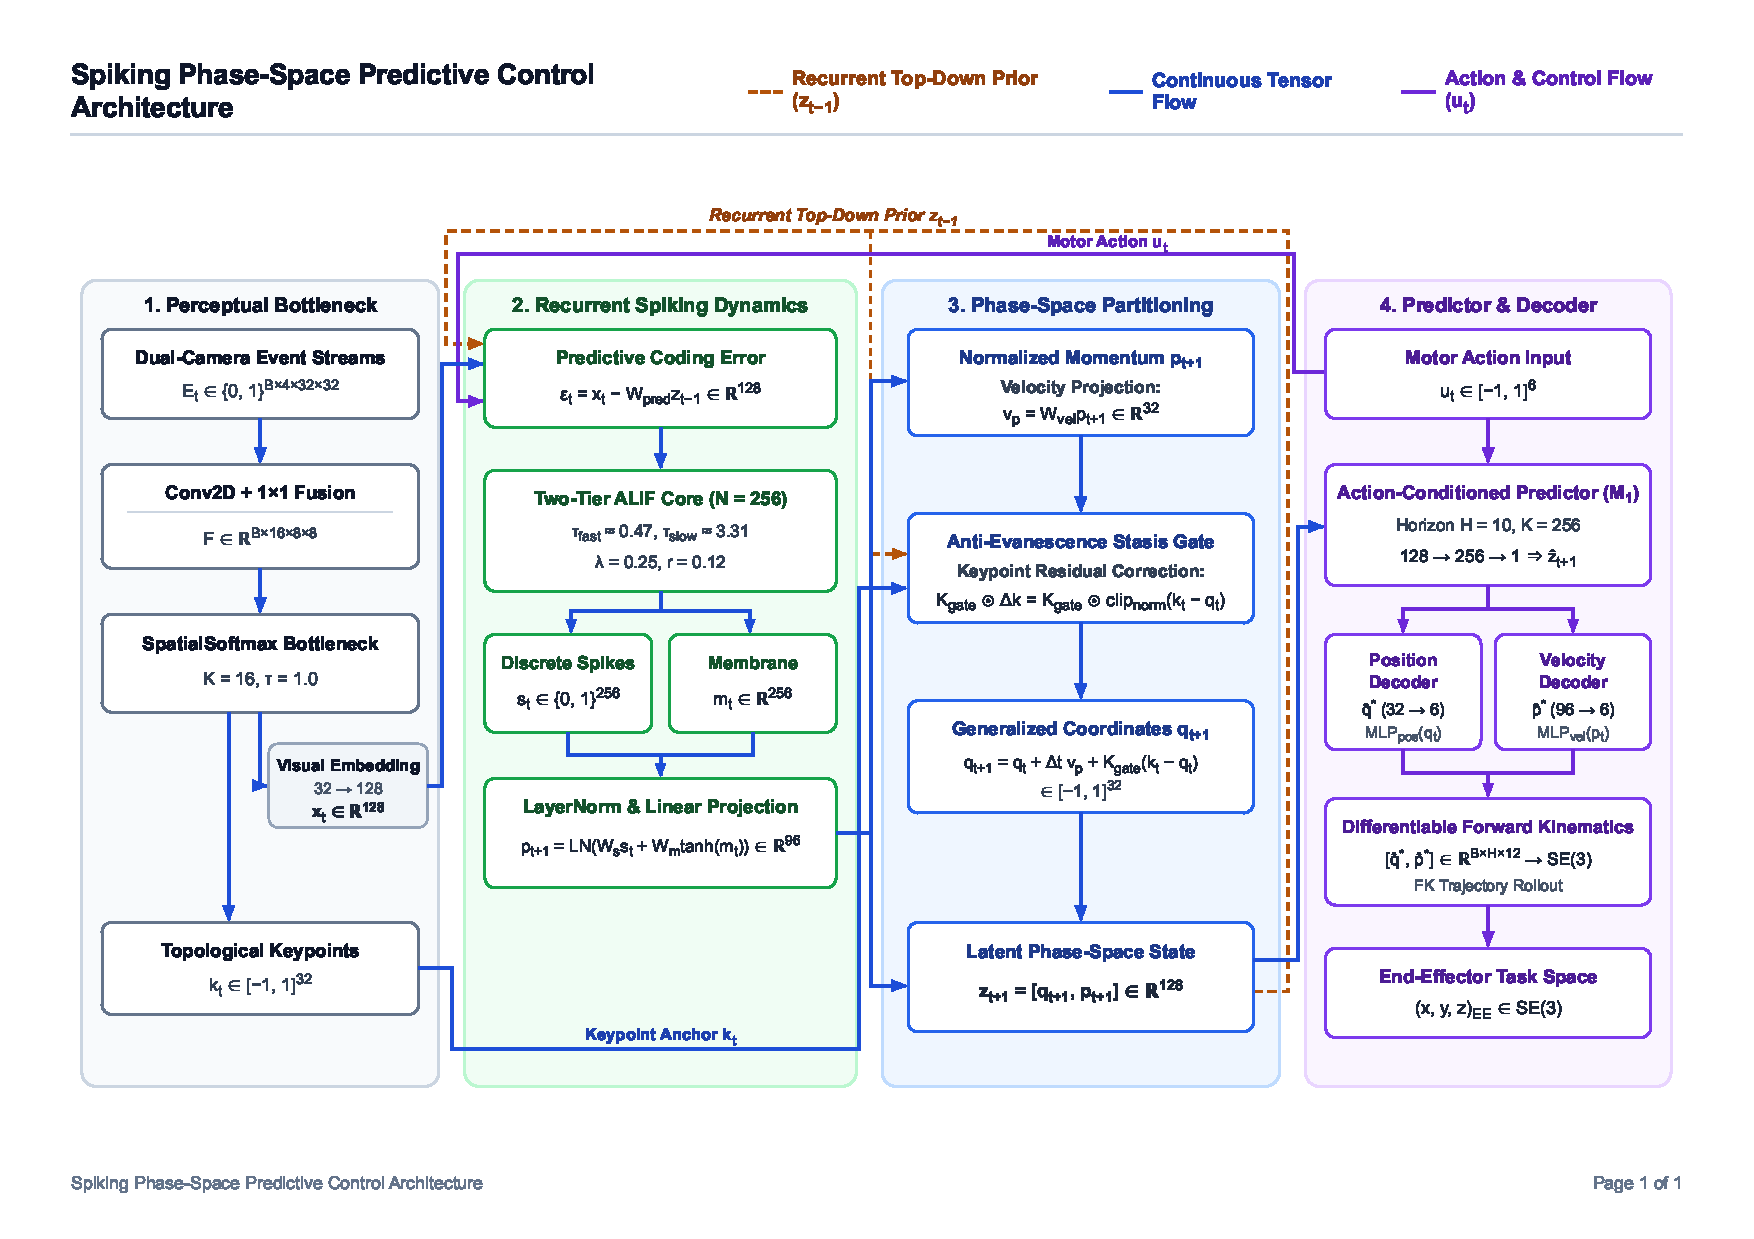
\includegraphics[width=0.78\textwidth]{architecture.pdf}
\caption{\textbf{End-to-End SPWM Architecture.} Four-stage dataflow: (1) \textit{Perceptual Bottleneck}: Dual event-camera streams $\mathbf{E}_t \in \{0, 1\}^{B \times 4 \times 32 \times 32}$ processed via Conv2D + residual wrist fusion ($\mathbf{F}_t \in \mathbb{R}^{B \times 16 \times 8 \times 8}$) and SpatialSoftmax ($\tau = 1.0$) extracting topological keypoints $\mathbf{k}_t \in [-1, 1]^{32}$ and visual embedding $\mathbf{x}_t \in \mathbb{R}^{128}$ ($15{,}904$ params); (2) \textit{Recurrent Spiking Dynamics}: Predictive coding error $\boldsymbol{\epsilon}_t = \mathbf{x}_t - \mathbf{W}_{\text{sens}}\mathbf{z}_{t-1}$ ($16{,}384$ params) and motor action $\mathbf{u}_t$ driving a two-tier ALIF core ($N=256$, reactive pool $\beta_1=0.90$ and deep pool $\beta_2=0.985$) with firing-rate homeostasis, producing spikes $\mathbf{s}_t \in \{0,1\}^{256}$ and membrane states $\mathbf{V}_t \in \mathbb{R}^{256}$; (3) \textit{Phase-Space Partitioning}: LayerNorm fusion into $\mathbf{p}_{t} \in \mathbb{R}^{96}$ and direct velocity slicing $\mathbf{v}_p = \mathbf{p}_{t}[..., :32]$ into $\mathbf{q}_{t} \in \mathbb{R}^{32}$ regulated by the Anti-Evanescence Stasis Gate $K_{\text{gate}}$ ($117{,}312$ active params); (4) \textit{Predictor \& Decoder}: Action-conditioned dissipative surrogate $M_1$ ($158{,}944$ params) and zero-lag kinematic decoder ($9{,}356$ params) feeding Differentiable Forward Kinematics (FK) and Residual-Gated Sensory Handover (Eq.~\ref{eq:handover}).}\label{fig:architecture}
\end{figure}

\subsection{Continuous-Time Latent POMDP and Dual-Camera Neuromorphic Encoding}
We model 3D articulated manipulation as a continuous-time POMDP embedded in $\mathcal{M} = \text{SE}(3) \times \mathbb{R}^J$ ($J=6$). At discrete control steps $\Delta t = 0.05\,\text{s}$ ($20\,\text{Hz}$) integrating over $100\,\text{Hz}$ physics sub-steps ($\Delta t_{\text{phys}} = 0.01\,\text{s}$), normalized motor commands $\mathbf{u}_t \in [-1.0, 1.0]^6$ (scaled by $\theta_{\max} = 3.14\,\text{rad}$) drive the manipulator across three task phases $\phi_t \in \{0, 1, 2\}$: \textit{Blind Approach} ($\phi_t = 0$), \textit{Sensory Heft} ($\phi_t = 1$, spanning a 14-step dataset window $[t_{\text{contact}}-7, t_{\text{contact}}+7)$ around dataset contact $t_{\text{contact}}$; in closed-loop PIL evaluation, $t_c$ indexes the $\phi_t=1$ sensory-window onset \texttt{p1\_indices[0]} $= t_{\text{contact}}-7$, where PIL engages the rigid payload load $\texttt{payload\_attached} = (t \ge t_c)$ with $m_{\text{payload}} \in [1.20, 4.50]\,\text{kg}$ and evaluates the 7-step loaded transition through $t_{\text{grasp}} = t_c + 7 = t_{\text{contact}}$), and \textit{Blind Transport} ($\phi_t = 2$).

To resolve axial wrist-roll symmetry and elbow-flex depth foreshortening, a dual-camera neuromorphic system ($C = 4$, $H = W = 32$, threshold $\theta = 0.08$) pairs a static global observer (channels 0..1) with an egocentric wrist-mounted camera (channels 2..3), yielding $\mathbf{E}_t \in \{0, 1\}^{B \times 4 \times 32 \times 32}$. The encoder $\mathcal{E}_\theta$ processes $\mathbf{E}_t$ through a two-stage stride-2 Conv2D + GroupNorm + SiLU backbone ($\text{channels } (16, 32) \to 16$ at $8 \times 8$), adds a dedicated egocentric wrist stem ($\text{Conv2D}(2 \to 16 \to 32) + 1 \times 1$ fusion head) via residual addition $\mathbf{F}_t = \text{conv}(\mathbf{E}_t) + \text{fusion}(\text{wrist\_stem}(\mathbf{E}_{t, 2:4})) \in \mathbb{R}^{B \times 16 \times 8 \times 8}$, extracts expected 2D keypoint coordinates $\mathbf{k}_t \in [-1, 1]^{32}$ via SpatialSoftmax \cite{finn2016spatial}, and projects via $\text{Linear}(32, 128) + \text{LayerNorm} + \text{SiLU}$ to $\mathbf{x}_t \in \mathbb{R}^{128}$ to form top-down predictive-coding residuals $\boldsymbol{\epsilon}_t = \mathbf{x}_t - \mathbf{W}_{\text{sens}}\mathbf{z}_{t-1}$.

\subsection{Recurrent Spiking Dynamics and Anti-Evanescence Stasis Gating}
The spiking dynamics module $\mathcal{F}_\theta$ factorizes the latent state into $\mathbf{z}_t = [\mathbf{q}_t, \mathbf{p}_t] \in \mathbb{R}^{128}$ ($\mathbf{q}_t \in \mathbb{R}^{32}$, $\mathbf{p}_t \in \mathbb{R}^{96}$). At each step, somatic current $\mathbf{I}_{\text{soma},t} = \mathbf{W}_{\text{in}}\boldsymbol{\epsilon}_t + \mathbf{W}_{\text{rec}}\mathbf{p}_{t-1} + \mathbf{W}_q\mathbf{q}_{t-1} + \mathbf{W}_u\mathbf{u}_t \in \mathbb{R}^{256}$ (with $\mathbf{W}_u$ zero-initialized so action coupling is learned cleanly from kinematic gradients) drives $N = 256$ ALIF neurons \cite{bellec2020solution} partitioned into reactive ($128$ units, $\beta_{\text{adapt},1} = 0.90$, $\tau_{\text{adapt}} \approx 0.47\,\text{s}$) and slow contextual ($128$ units, $\beta_{\text{adapt},2} = 0.985$, $\tau_{\text{adapt}} \approx 3.31\,\text{s}$) pools:
\begin{equation}
\begin{aligned}
\mathbf{V}_t &= \beta_{\text{mem}}\mathbf{V}_{t-1} + \mathbf{I}_{\text{soma},t} - \mathbf{s}_{t-1}V_{\text{th0}}, \quad
\mathbf{A}_t = \beta_{\text{adapt}}\mathbf{A}_{t-1} + \mathbf{s}_{t-1}, \\
\mathbf{s}_t &= \Theta\!\left(\mathbf{V}_t - (V_{\text{th0}} + \gamma \mathbf{A}_t)\right),
\end{aligned}
\end{equation}
with learnable per-neuron decays clamped to $\beta_{\text{mem}} \in [0.50, 0.98]$ (init $0.80$) and $\beta_{\text{adapt}} \in [0.80, 0.995]$, $\gamma=0.18$, $V_{\text{th0}}=1.0$, and Arctangent surrogate derivative $\partial s / \partial x = (\alpha/2) / (1 + (\frac{\pi}{2}\alpha x)^2)$ ($\alpha=2.0$). Firing-rate homeostasis prevents silent-neuron collapse and energetic saturation:
\begin{equation}
\mathcal{L}_{\text{spike\_bal}} = \sum_{i=1}^{N}(\bar{s}_i - r_{\text{target}})^2 + 4\sum_{i=1}^{N}\max(0, 0.02 - \bar{s}_i)^2 + 2\sum_{i=1}^{N}\max(0, \bar{s}_i - 0.45)^2,
\end{equation}
with $r_{\text{target}} = 0.12$ and $\lambda_{\text{spike\_balance}} = 0.25$ ($\mathcal{L}_{\text{spike\_balance}} \equiv \mathcal{L}_{\text{spike\_bal}}$). Generalized momentum updates via $\mathbf{p}_{t} = \text{LN}(\mathbf{W}_{\text{sp}}\mathbf{s}_t + \mathbf{W}_{\text{mem}}\tanh(\mathbf{V}_t)) \in \mathbb{R}^{96}$, and coordinate velocity is extracted by direct subspace slicing $\mathbf{v}_p = \mathbf{p}_t[..., :32]$.

Because differential event cameras emit zero events when the arm pauses ($a_t \to 0$), residual currents from the slow ALIF pool would otherwise cause stationary coordinate drift. We solve this event-stasis paradox by gating coordinate integration with dual-stream maximum event activity $a_t = \max(\overline{|\mathbf{E}_{t,\text{global}}|}, \overline{|\mathbf{E}_{t,\text{wrist}}|})$ ($\sigma_{\text{stasis}}=0.003$, $a_{\text{thresh}}=0.001$, $a_{\text{eff}} = \max(0, a_t - a_{\text{thresh}})$), consecutive active-step counter $g_t = \mathbb{I}[a_t > a_{\text{thresh}}](g_{t-1} + 1)$ with ramp $\rho_t = \operatorname{clamp}(g_t / N_{\text{ramp}}, 0, 1)$ ($N_{\text{ramp}}=4$), and Anti-Evanescence Stasis Gate $K_{\text{gate}} \in [0, K_{\text{max}}]^{32}$ ($K_{\text{max}} = 0.35$):
\begin{align}
K_{\text{gate}} &= \operatorname{clamp}\!\left(\rho_t K_{\text{max}}\!\left(1 - e^{-\operatorname{softplus}(\mathbf{g}_{\text{scale}}) a_{\text{eff}}}\right)\! \odot \tanh^2\!\left(\frac{a_{\text{eff}}}{\sigma_{\text{stasis}}}\right),\, 0,\, K_{\text{max}}\right), \\
\mathbf{q}_{t} &= \mathbf{q}_{t-1} + \Delta t \tanh\!\left(\frac{a_t}{\sigma_{\text{stasis}}}\right)\mathbf{v}_p + K_{\text{gate}} \odot \text{clip}_{\text{norm}}\!\left(\mathbf{k}_t - \mathbf{q}_{t-1}, \, 0.50\right),
\end{align}
where $\mathbf{g}_{\text{scale}} \in \mathbb{R}^{32}$ is initialized to $50.0$ (converging to $49.04\text{--}49.07$ across seeds).

\subsection{Dissipative Attractor Surrogate ($M_1$) and Residual-Gated Latent MPPI}
Unlike conservative systems where strict skew-symmetric recurrence preserves phase-space volume, 6-DOF manipulation under joint friction and variable payload inertia ($1.20\text{--}4.50\,\text{kg}$) is inherently dissipative. The differentiable continuous surrogate $M_1$ parameterizes a state-dependent dissipative vector field optimized for batched GPU/NPU MPPI rollouts. Given $\mathbf{h}_t = \text{MLP}_{\text{backbone}}([\mathbf{z}_t, \mathbf{u}_t]) \in \mathbb{R}^{256}$ (two $\text{Linear} + \text{LayerNorm} + \text{SiLU}$ layers), $M_1$ predicts generalized forces $\mathbf{f}_p \in \mathbb{R}^{96}$, state-dependent dissipation $\boldsymbol{\gamma}_t \in (0, 1)^{96}$ (bias initialized to $-2.0$), and restorative coordinate drift $\mathbf{f}_q \in \mathbb{R}^{32}$ (zero-initialized):
\begin{align}
\mathbf{f}_p &= \mathbf{W}_p \mathbf{h}_t + \mathbf{b}_p, \qquad \boldsymbol{\gamma}_t = \sigma(\mathbf{W}_\gamma \mathbf{h}_t + \mathbf{b}_\gamma), \qquad \mathbf{f}_q = \mathbf{W}_q \mathbf{h}_t + \mathbf{b}_q, \\
\hat{\mathbf{p}}_{t+1} &= (1 - \Delta t \cdot \boldsymbol{\gamma}_t) \odot \mathbf{p}_t + \mathbf{f}_p, \qquad
\hat{\mathbf{q}}_{t+1} = \mathbf{q}_t + \Delta t \cdot \left(\hat{\mathbf{p}}_{t+1}[..., :32] + \mathbf{f}_q\right).
\end{align}
The zero-lag kinematic decoder $\mathcal{D}_\theta$ ($\alpha_{\text{pos}}=\alpha_{\text{vel}}=0.0$, two 64-unit SiLU MLPs) maps $\mathbf{q}_t \mapsto \hat{\mathbf{q}}_t^* \in \mathbb{R}^6$ and $\mathbf{p}_t \mapsto \hat{\mathbf{p}}_t^* \in \mathbb{R}^6$.

In closed-loop execution, the Latent MPPI planner ($K=256$, $H=10$, $N_{\text{iter}}=3$, $\lambda=0.20$, $\gamma_{\text{nom}}=0.60$) evaluates candidate trajectories over a \textbf{2-Stage $\text{SE}(3)$ Lookahead} ($\mathbf{T}^*_{\text{plan}}(t+\tau) = \mathbf{T}^*_{\text{grasp}}$ for $t+\tau \le t_c$ and $\mathbf{T}^*_{\text{final}}$ for $t+\tau > t_c$), sampling AR(1) perturbations ($\beta=0.90$, $\sigma=0.08$, shoulder $1.6\times$, elbow $1.4\times$) with action slew-rate clamping ($\|\Delta \mathbf{u}\|_\infty \le 0.10$) and minimizing:
\begin{equation}\label{eq:mppi_cost}
\begin{aligned}
\mathcal{C}_k &= \sum_{h=1}^{H}\Big[w_{\text{pos}}e_{\text{pos},h} + w_{\text{rot}}\big((1-\cos\theta_h) + 0.5\theta_h\big) + w_{\text{jerk}}\|\Delta\mathbf{u}_h\|_2^2\Big] \\
&\quad + \sum_{h=1}^{H}\Big[-w_{\text{prog}}\alpha_h(\Delta\mathbf{p}_{\text{ee},h}\!\cdot\!\hat{\mathbf{d}}_h) + w_{\text{damp}}(1-\alpha_h)\|\Delta\mathbf{p}_{\text{ee},h}\|_2\Big] \\
&\quad + \sum_{h=1}^{H}\Big[w_{\text{accel}}\|\Delta^2\hat{\mathbf{q}}^*_h\|_2^2 + w_{\text{limit}}\big\|\operatorname{ReLU}(\hat{\mathbf{q}}^*_h - \mathbf{q}_{\max}) + \operatorname{ReLU}(\mathbf{q}_{\min} - \hat{\mathbf{q}}^*_h)\big\|_2^2\Big],
\end{aligned}
\end{equation}
with deadband factor $\alpha_h = \operatorname{clamp}((e_{\text{pos},h} - 0.03)/0.10, 0, 1)$, $w_{\text{pos}}=80$, $w_{\text{rot}}=100$, $w_{\text{prog}}=50$, $w_{\text{damp}}=12$, $w_{\text{jerk}}=4$, $w_{\text{accel}}=15$, $w_{\text{limit}}=50$, and $w_{\text{critic}}=0$ at inference. Because unconditional mid-trajectory sensory re-injection perturbs $M_1$'s momentum manifold during open-loop unrolls, SPWM employs \textbf{Residual-Gated Sensory Handover} strictly as a quality-verified closed-loop state-correction gate during $\phi_t = 1$:
\begin{equation}\label{eq:handover}
\begin{aligned}
\mathbf{z}_{t+1} &= (1 - w_t)\,\hat{\mathbf{z}}_{t+1} + w_t\,\mathbf{z}^{\text{obs}}_{t+1}, \\
w_t &= \begin{cases}
0.85, & d_{\text{pred}} > \tau \wedge d_{\text{obs}} < 0.025 \wedge \theta_{\text{obs}} < 0.049, \\
0.40\,\eta_t, & \text{else if } d_{\text{obs}} < d_{\text{pred}} \wedge t \le t_c + 2, \\
0.0, & \text{otherwise},
\end{cases}
\end{aligned}
\end{equation}
where $\tau = 0.026\,\text{m}$ default, $\eta_t = \operatorname{clamp}((d_{\text{pred}} - 0.032)/0.04, 0, 1)$, $\hat{\mathbf{z}}_{t+1} = M_1(\mathbf{z}_t, \mathbf{u}_t)$, $\mathbf{z}^{\text{obs}}_{t+1}$ is the online ALIF-grounded state, and $(d_{\text{pred}}, d_{\text{obs}}, \theta_{\text{obs}})$ are the decoded FK end-effector position (m) and $\text{SO}(3)$ orientation (rad) errors relative to $\mathbf{T}^*_{\text{final}}$.

\subsection{Decoupled Two-Phase Curriculum}
\textbf{Phase 0: Grounded State Estimation (160 epochs).} $M_1$ and the latent critic are frozen. Three learning-rate tiers across five Adam parameter groups (\texttt{encoder}, non-$\beta_*$ \texttt{dynamics}, and \texttt{sensory\_predictor} at $10^{-4}$; $\beta_*$ at $5\times 10^{-5}$ with zero weight decay; \texttt{physical\_decoder} at $2\times 10^{-4}$; cosine decay to $0.20\times$) optimize $\mathcal{L}_{\text{Phase 0}} = 5.0\mathcal{L}_{\text{kin}} + 1.0\mathcal{L}_{\text{deriv}} + 0.1\mathcal{L}_{\text{smooth}} + 0.5\mathcal{L}_{\text{kin\_smooth}} + 0.25\mathcal{L}_{\text{spike\_bal}} + 1.0\mathcal{L}_{\text{sensory}}$.
\textbf{Phase 1: Action-Conditioned Attractor Learning (240 epochs; 260 on Seed 2024).} Phase 0 modules are frozen via strict scoped checkpoint loading. Adam ($\text{lr}=10^{-4}$, dropping to $5\times 10^{-5}$ in Latch Phase 4) updates $M_1$ and the latent critic over $H=100$ unrolls with half-open contact-heft weighting ($2.0\times$ on $\mathbf{q}$ over $[h_0-5, h_{\text{end}}+10)$ and $3.0\times$ on $\mathbf{p}$ over $[h_0, h_{\text{end}}+12)$) across four irreversible latch stages triggered by $\mathcal{L}_{M_1,\text{latent}}$: (1) Warmup ($w_t=0.60, \alpha=0 \to$ Phase 2 at $\mathcal{L}_{M_1,\text{latent}} < 0.10$), (2) Sensory Fade-Out ($w_t: 0.60 \to 0$ over 7 epochs $\to$ Phase 3 at $\mathcal{L}_{M_1,\text{latent}} < 0.095$), (3) AR(1) Noise Ramp ($\alpha: 0 \to 0.25$ over 20 epochs), and (4) DAgger Replay (\texttt{ClosedLoopBuffer}, 3-generation window, ratio $0.10 \to 0.50$).

\section{Experimental Setup}

Trajectories are generated in a Unity 6 (\texttt{6000.5.7f1}) PhysX 4 Featherstone 6-DOF environment with procedural rigid payloads (Sphere, Box, Elongated Cylinder; $1.20\text{--}4.50\,\text{kg}$) across three elevation planes (Low $1.04\,\text{m}$, Mid $1.14\,\text{m}$, High $1.26\,\text{m}$). The dataset comprises 4{,}000 trajectories ($T=105$ steps at $20\,\text{Hz}$ over $100\,\text{Hz}$ sub-steps), partitioned deterministically by ID into Train `[0, 3200)`, Validation `[3200, 3600)`, and Test `[3600, 4000)`. All closed-loop benchmarks execute strictly in \textbf{Physics-in-the-Loop (PIL)} on 50 unseen test episodes (`[3600, 3649]`): at each step $t$, decoded $(\mathbf{q}_{\text{des}}, \dot{\mathbf{q}}_{\text{des}})$ drive an analytical 100\,Hz decoupled 6-DOF articulated dynamics stepper (\texttt{ArticulatedArmPhysicsStepper}, diagonal effective inertia, $K_{\text{stiff}}=16.5$, $k_p=18.0$, $k_d=0.80$, Coulomb friction $0.04\tanh(5\mathbf{p})$, symmetric $[-\pi, \pi]$ joint limits) with causal payload attachment $\texttt{payload\_attached} = (t \ge t_c)$ and causal online dual-camera event rendering (\texttt{OnlineEventCameraStream}), with zero access to ground-truth future latents. Payload attachment is modeled as a rigid palm-latch (\texttt{FixedJoint} in Unity; $\texttt{payload\_attached} = (t \ge t_c)$ in PIL) rather than multi-finger friction contact. An episode counts as a grasp success iff end-effector position error stays $< 3.0\,\text{cm}$ across the final 3-step settling window, terminal $\text{SO}(3)$ orientation error satisfies $\theta_{\text{final}} < 0.05\,\text{rad}$, and terminal joint velocity satisfies $\|\dot{\mathbf{q}}(t_{\text{grasp}})\|_2 < \max(1.5, 1.1\|\dot{\mathbf{q}}^*_{t_{\text{grasp}}}\|_2)\,\text{rad/s}$. We compare SPWM ($392.1\text{k}$ total / $317.9\text{k}$ active params, 3 seeds) against parameter-matched \texttt{ANN-Rate} ($392.1\text{k} / 317.9\text{k}$, 3 seeds), Continuous RSSM ($380.5\text{k}$, 3 seeds, evaluated under \textit{both} Open-Loop PIL and Online Posterior updates during $\phi_t=1$), Deep GRU ($338.9\text{k}$, 3 seeds, Open-Loop and Online), Continuous ConvLSTM ($296.9\text{k}$), Reactive Behavior Cloning ($322.2\text{k}$ params), and a non-learned \textit{Privileged State-Oracle Jacobian-IK + PD} controller that reads true physical joint angles $\mathbf{q}_{\text{phys}}$ directly (bypassing the event cameras and partial observability) with fixed gains calibrated to the mean training payload mass ($2.85\,\text{kg}$).

\section{Results and Analysis}

\subsection{Multi-Horizon Open-Loop Rollout Stability}
Table~\ref{tab:open_loop_rollout} reports multi-horizon open-loop rollout accuracy across all five frozen architectures on the $N=400$ unseen test split (`[3600, 3999]`, $t_{\text{start}}=4$, $H=100$). Across 3 seeds ($42, 101, 2024$), SPWM achieves the lowest long-horizon velocity MSE at $H=100$ ($0.00971 \pm 0.00177\,\text{rad}^2/\text{s}^2$)---a $2.16\times$ reduction over 3-seed Continuous RSSM ($0.02101 \pm 0.00044$), $11.5\times$ below Deep GRU ($0.11191$), and $34.7\times$ below Continuous ConvLSTM ($0.33696$)---while maintaining $0.00240 \pm 0.00037\,\text{rad}^2$ position MSE at $H=100$ (with $H=10$ exceeding $H=100$ because $t_{\text{start}}=4$ places $h=10$ at $t=14$ during the high-acceleration approach/contact transient before the dissipative attractor settles). On Canonical Seed 42 (Figure~\ref{fig:rollout_handover}), Pure Open-Loop $M_1$ unrolling yields $0.1115\,\text{rad}$ mean L2 joint error over $h \in [1, 100]$ at a $12.27\%$ ALIF spike rate, whereas unconditional Phasic Sensory Handover degrades tracking to $0.1482\,\text{rad}$ ($0.1827\,\text{rad}$ at $h=80$), confirming that un-gated mid-trajectory sensory injection perturbs $M_1$'s momentum manifold.

\begin{table}[t]
\centering
\caption{\textbf{Multi-Horizon Open-Loop Rollout ($N=400$ Test Trajectories `[3600, 3999]`, $H=100$, $t_{\text{start}}=4$).} Symmetric Position ($\text{rad}^2$) and Velocity ($\text{rad}^2/\text{s}^2$) MSE across horizons $H \in \{1, 10, 50, 100\}$. Mean $\pm$ seed std across 3 seeds ($42, 101, 2024$) for SPWM ($160+240$ ep on Seeds 42/101; $160+260$ ep on Seed 2024, best checkpoint at Ep 130), \texttt{ANN-Rate} ($160+240$ ep), and Continuous RSSM (60 end-to-end epochs/seed); Seed 42 for Deep GRU (59 ep) and Continuous ConvLSTM (54 ep).}
\label{tab:open_loop_rollout}
\scriptsize
\setlength{\tabcolsep}{3.5pt}
\resizebox{\textwidth}{!}{%
\begin{tabular}{lccccccccc}
\toprule
\textbf{Model Architecture} & \textbf{Params (Act.)} & \textbf{Pos H=1} & \textbf{Pos H=10} & \textbf{Pos H=50} & \textbf{Pos H=100} & \textbf{Vel H=1} & \textbf{Vel H=10} & \textbf{Vel H=50} & \textbf{Vel H=100} \\
\midrule
Continuous ConvLSTM & 296.9k & 0.00002 & \textbf{0.00012} & \textbf{0.00150} & 0.00707 & 0.00147 & \textbf{0.00553} & \textbf{0.01095} & 0.33696 \\
Deep GRU & 338.9k & 0.00003 & 0.00029 & 0.00173 & 0.00650 & 0.00097 & 0.00643 & 0.01605 & 0.11191 \\
Continuous RSSM (3 seeds) & 380.5k & \textbf{0.00001 $\pm$ 0.00001} & 0.00029 $\pm$ 0.00006 & 0.00166 $\pm$ 0.00002 & \textbf{0.00145 $\pm$ 0.00009} & \textbf{0.00033 $\pm$ 0.00017} & 0.01659 $\pm$ 0.00244 & 0.02262 $\pm$ 0.00088 & 0.02101 $\pm$ 0.00044 \\
ANN-Rate (Leaky, 3 seeds) & 392.1k (317.9k) & 0.00028 $\pm$ 0.00012 & 0.00249 $\pm$ 0.00032 & 0.00341 $\pm$ 0.00264 & 0.00210 $\pm$ 0.00063 & 0.00193 $\pm$ 0.00069 & 0.03356 $\pm$ 0.00511 & 0.02440 $\pm$ 0.01698 & 0.01183 $\pm$ 0.00715 \\
\textbf{SPWM (Ours, 3 seeds)} & \textbf{392.1k (317.9k)} & 0.00018 $\pm$ 0.00011 & 0.00348 $\pm$ 0.00265 & 0.00315 $\pm$ 0.00144 & 0.00240 $\pm$ 0.00037 & 0.00139 $\pm$ 0.00076 & 0.04507 $\pm$ 0.02601 & 0.02466 $\pm$ 0.01271 & \textbf{0.00971 $\pm$ 0.00177} \\
\bottomrule
\end{tabular}%
}
\end{table}

\begin{figure}[t]
\centering
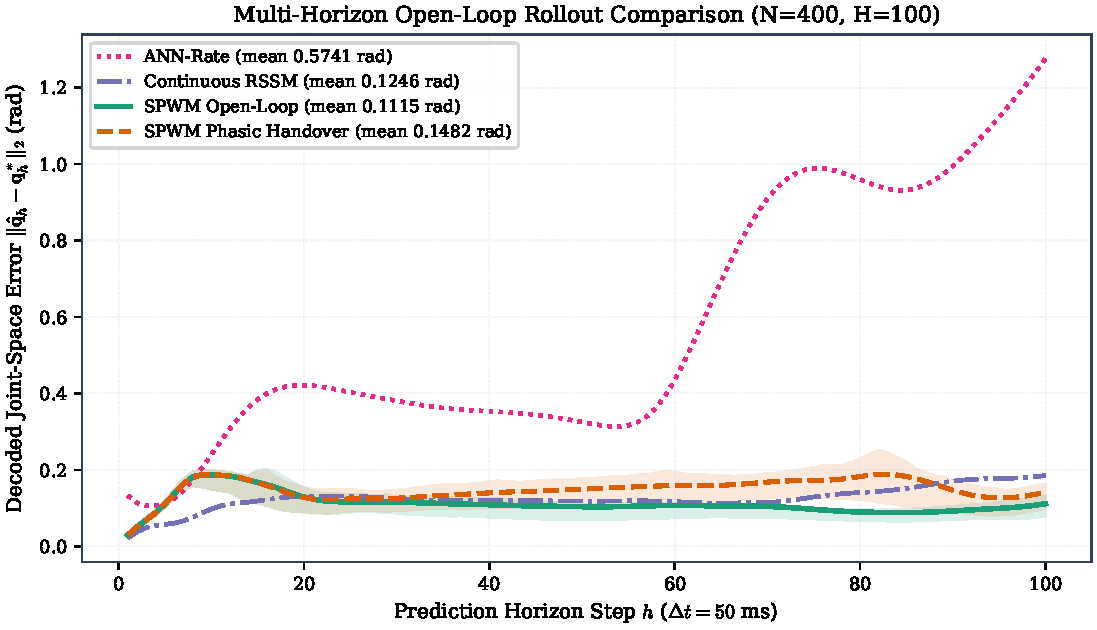
\includegraphics[width=0.62\textwidth]{fig2_rollout_open_vs_handover.pdf}
\caption{\textbf{Multi-Horizon Rollout: Open-Loop vs.\ Phasic Handover ($N=400$, $H=100$).} Decoded joint-space L2 error $\|\hat{\mathbf{q}}_h - \mathbf{q}^*_h\|_2$ (mean $\pm$ IQR) across 400 unseen test trajectories at $12.27\%$ measured ALIF spike rate. SPWM Pure Open-Loop ($0.1115\,\text{rad}$ mean; $0.0899\,\text{rad}$ at $h=80$, $0.1116\,\text{rad}$ at $h=100$) avoids the late-horizon divergence of un-gated Phasic Sensory Handover ($0.1482\,\text{rad}$ mean; $0.1827\,\text{rad}$ at $h=80$).}\label{fig:rollout_handover}
\end{figure}

\subsection{Closed-Loop Physics-in-the-Loop Control \& Forensic Failure Analysis}
Across the 50 unseen PIL test episodes (`[3600, 3649]`, Table~\ref{tab:pil_control} and Figure~\ref{fig:mppi_bench}), SPWM achieves \textbf{86.0\% (43/50)} grasp success on Canonical Seed 42 ($0.86 \pm 0.80\,\text{cm}$ min error, $1.57 \pm 1.00\,\text{cm}$ terminal error, $|\Delta^2 q| = 0.00587\,\text{rad/step}^2$), stratifying to $86.4\%$ Low ($22$ ep, $0.86\,\text{cm}$), $77.8\%$ Mid ($18$ ep, $1.05\,\text{cm}$), and $100.0\%$ High ($10$ ep, $0.50\,\text{cm}$) across elevation planes, and $82.4\%$ Light ($17$ ep, $0.68\,\text{cm}$), $100.0\%$ Medium ($17$ ep, $0.77\,\text{cm}$), and $75.0\%$ Heavy ($16$ ep, $1.14\,\text{cm}$) across mass tiers. Across all 3 seeds, SPWM achieves \textbf{58.0 $\pm$ 27.1\%} under original $N=6$ Tier-2 validation selection (`86.0% / 56.0% / 32.0%`) and \textbf{60.7 $\pm$ 2.3\%} (`58.0% / 62.0% / 62.0%`, $0.88 \pm 0.11\,\text{cm}$ min error, $2.01 \pm 0.12\,\text{cm}$ terminal error) when selecting among the 5 saved phase checkpoints per seed using $N=25$ held-out validation episodes (`[3200, 3224]`; Appendix Table~\ref{tab:forensic_diagnostics}b)---reducing inter-seed test std by \textbf{11.7$\times$} with zero test-set peeking.

\begin{table}[t]
\centering
\caption{\textbf{Closed-Loop Physics-in-the-Loop (PIL) Manipulation Benchmark (`50` Test Episodes `[3600, 3649]`, Payload Attached at Sensory-Window Onset $t \ge t_c$, $t_{\text{grasp}} = t_c + 7$).} Continuous recurrent baselines (RSSM, Deep GRU) are reported under \textit{both} Open-Loop PIL (no sensory overwrite during $\phi_t=1$) and Online Observation Update during $\phi_t=1$. SPWM is reported under $N=6$ Tier-2 checkpoint selection, expanded $N=25$ validation-split (`[3200, 3224]`) selection, and Canonical Seed 42. $^*$Unthrottled CPU latency (from \texttt{multiseed\_metrics.json} / \texttt{physics\_in\_loop/spwm/}); primary values for SPWM, Open-Loop RSSM, and Open-Loop Deep GRU reflect 2-thread \texttt{OMP\_NUM\_THREADS=2} evaluation, while Online RSSM, Online Seed-42 Deep GRU, \texttt{ANN-Rate}, and Oracle PD / Reactive BC ran unthrottled ($^\dagger$mixed unthrottled Seed 42 and 2-thread Seeds 101/2024).}
\label{tab:pil_control}
\scriptsize
\setlength{\tabcolsep}{3.5pt}
\resizebox{\textwidth}{!}{%
\begin{tabular}{lccccccc}
\toprule
\textbf{Method} & \textbf{PIL Success (\%)} & \textbf{Min Err (cm)} & \textbf{Term Err (cm)} & $|\Delta^2 q|$ ($\text{rad/step}^2$) & $|\Delta^3 q|$ & \textbf{Flips} & \textbf{Latency (ms)} \\
\midrule
\textit{Privileged State-Oracle Jacobian-IK + PD ($\mathbf{q}_{\text{phys}}$, no vision, 2.85\,kg cal.)} & \textit{96.0} & \textit{0.01 $\pm$ 0.03} & \textit{0.43 $\pm$ 0.73} & \textit{0.00771} & \textit{0.00497} & \textit{10.46} & \textit{22.7$^*$} \\
\midrule
Reactive BC (50 ep, Seed 42, 322.2k) & 0.0 & 13.13 $\pm$ 6.27 & 15.66 $\pm$ 8.15 & 0.00140 & 0.00135 & 13.98 & 1.9$^*$ \\
Deep GRU (Open-Loop PIL, 3 seeds) & 1.3 $\pm$ 2.3 & 10.57 $\pm$ 7.83 & 16.72 $\pm$ 11.31 & 0.00777 & 0.00622 & 14.67 & 67.4 \\
Deep GRU (Online Obs., 3 seeds) & 0.0 $\pm$ 0.0 & 6.03 $\pm$ 4.00 & 10.87 $\pm$ 3.97 & 0.01654 & 0.01350 & 19.67 & 60.3$^\dagger$ \\
Continuous RSSM (Open-Loop PIL, 3 seeds) & 15.3 $\pm$ 4.6 & 1.31 $\pm$ 0.02 & 2.88 $\pm$ 0.10 & 0.01998 & 0.02059 & 36.23 & 52.4 \\
Continuous RSSM (Online Post., 3 seeds) & 0.0 $\pm$ 0.0 & 1.53 $\pm$ 0.06 & 22.43 $\pm$ 0.58 & 0.03119 & 0.02875 & 36.13 & 35.1$^*$ \\
ANN-Rate (Leaky Rate, 3 seeds) & 37.3 $\pm$ 9.5 & 1.07 $\pm$ 0.28 & 2.98 $\pm$ 0.46 & 0.01148 & 0.00938 & 26.00 & 24.6$^*$ \\
\textbf{SPWM ($N=6$ Tier-2, 3 seeds)} & \textbf{58.0 $\pm$ 27.1} & \textbf{0.90 $\pm$ 0.04} & \textbf{2.23 $\pm$ 0.68} & \textbf{0.00860} & \textbf{0.00608} & \textbf{19.37} & \textbf{27.5 (23.1$^*$)} \\
\textbf{SPWM ($N=25$ Val-Sel., 3 seeds)} & \textbf{60.7 $\pm$ 2.3} & \textbf{0.88 $\pm$ 0.11} & \textbf{2.01 $\pm$ 0.12} & \textbf{0.00931} & \textbf{0.00663} & \textbf{21.14} & \textbf{35.5} \\
\textbf{SPWM (Canonical Seed 42)} & \textbf{86.0} & \textbf{0.86 $\pm$ 0.80} & \textbf{1.57 $\pm$ 1.00} & \textbf{0.00587} & \textbf{0.00354} & \textbf{14.02} & \textbf{36.7 (23.3$^*$)} \\
\bottomrule
\end{tabular}%
}
\end{table}

\begin{figure}[t]
\centering
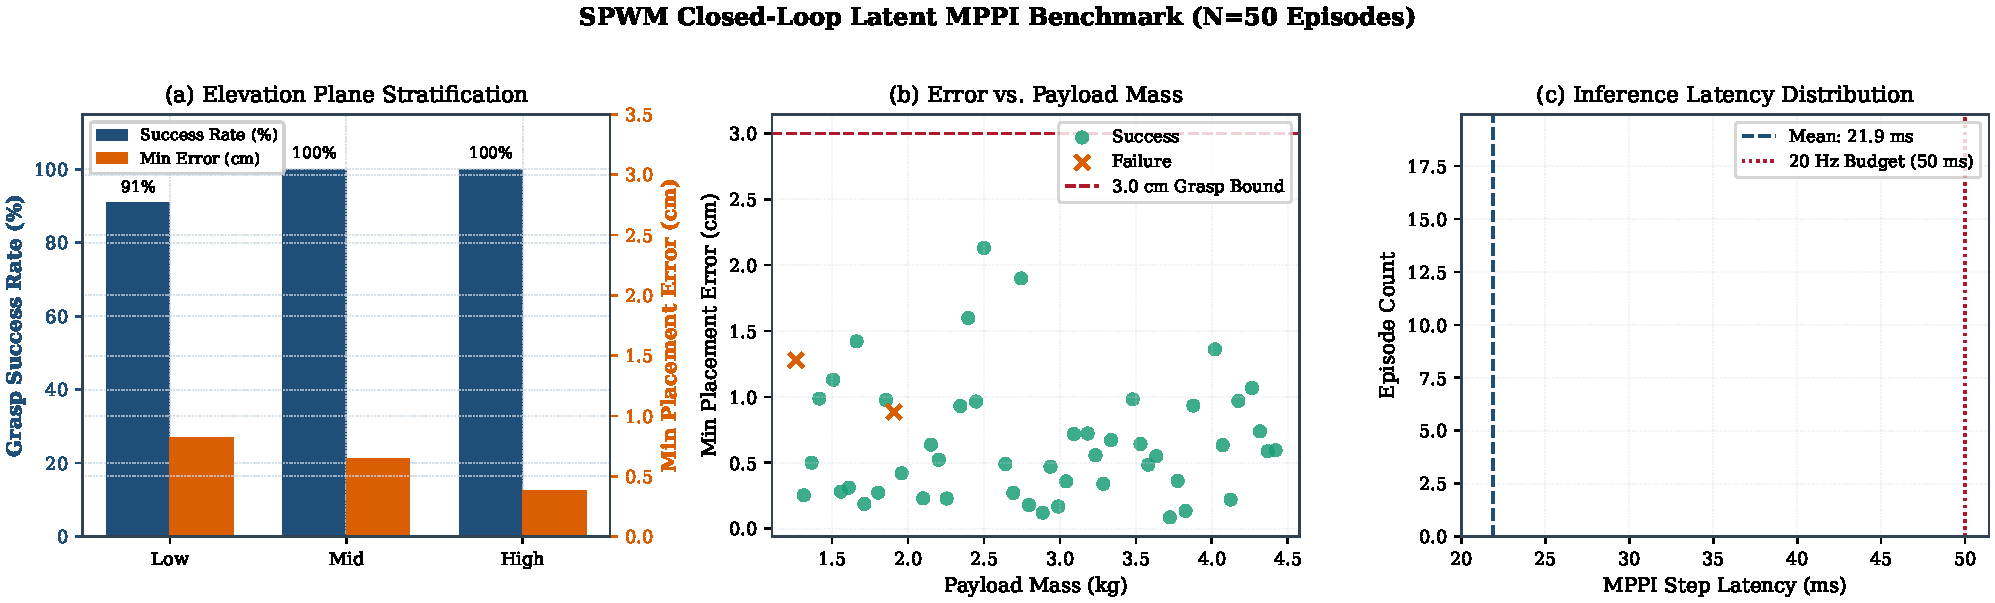
\includegraphics[width=0.78\textwidth]{fig1_mppi_benchmark.pdf}
\caption{\textbf{Closed-Loop Latent MPPI 50-Episode PIL Benchmark (SPWM Seed 42, $86.0\%$ Overall).} (a) Stratification across elevation planes ($86.4\%$ Low, $77.8\%$ Mid, $100.0\%$ High), with Grasp Success Rate (\%) and Min Placement Error (cm); (b) Minimum placement error vs.\ payload mass ($0.86 \pm 0.80\,\text{cm}$ overall; $82.4\%$ Light, $100.0\%$ Medium, $75.0\%$ Heavy); (c) Inference latency distribution ($36.7\,\text{ms}$ under 2-thread CPU limit; $23.3\,\text{ms}$ unthrottled).}\label{fig:mppi_bench}
\end{figure}

\textbf{Forensic Root Cause of Continuous RSSM \& Deep GRU Collapse (Figure~\ref{fig:heft_shock}):} Despite achieving competitive open-loop position MSE ($0.00145\,\text{rad}^2$ at $H=100$), Continuous RSSM scores $0.0\%$ across all 150 online PIL episodes ($3\text{ seeds} \times 50\text{ ep}$) and only $15.3 \pm 4.6\%$ in Open-Loop PIL (`18.0% / 10.0% / 18.0%`). Forensic decomposition (Appendix Table~\ref{tab:forensic_diagnostics}a) reveals that RSSM successfully guides the end-effector within $\le 3.0\,\text{cm}$ of the target pre-contact in \textbf{141/150 (94.0\%)} episodes ($49/50 = 98.0\%$ on Seed 42, reaching $1.58\,\text{cm}$ pre-$t_c$ min error and $3.13\,\text{cm}$ at $t_c$). However, immediately after $t_c$ when the rigid payload inertia attaches and online event bursts update the recurrent posterior ($w_t=1.0$), RSSM suffers \textbf{141/150 post-contact impulse divergence + velocity violations} ($100\%$ of the reaching episodes), with Seed 42 error exploding from $3.13\,\text{cm}$ at $t_c$ to $23.06 \pm 10.19\,\text{cm}$ at $t_{\text{grasp}} = t_c + 7$ and terminal velocity reaching $7.41 \pm 1.42\,\text{rad/s}$ ($7.17 \pm 0.32\,\text{rad/s}$ 3-seed mean, exceeding the $1.50\,\text{rad/s}$ stability threshold by $4.8\times$). Conversely, SPWM's dissipative attractor $M_1$ and ALIF thresholding absorb the contact shock, contracting error from $1.69\,\text{cm}$ at $t_c$ to $1.57\,\text{cm}$ at $t_{\text{grasp}}$ with $0.33 \pm 0.25\,\text{rad/s}$ terminal velocity ($0/50$ velocity violations) and $3.4\times$ lower joint acceleration than Open-Loop RSSM ($0.00587$ vs.\ $0.01998\,\text{rad/step}^2$ on Seed 42; $2.3\times$ lower across 3-seed $N=6$ at $0.00860$). Similarly, parameter-matched \texttt{ANN-Rate} ($37.3 \pm 9.5\%$) suffers $19/50$ post-contact spatial divergences on Seed 42 ($34.0\%$) due to sub-threshold continuous rate drift.

\begin{figure}[t]
\centering
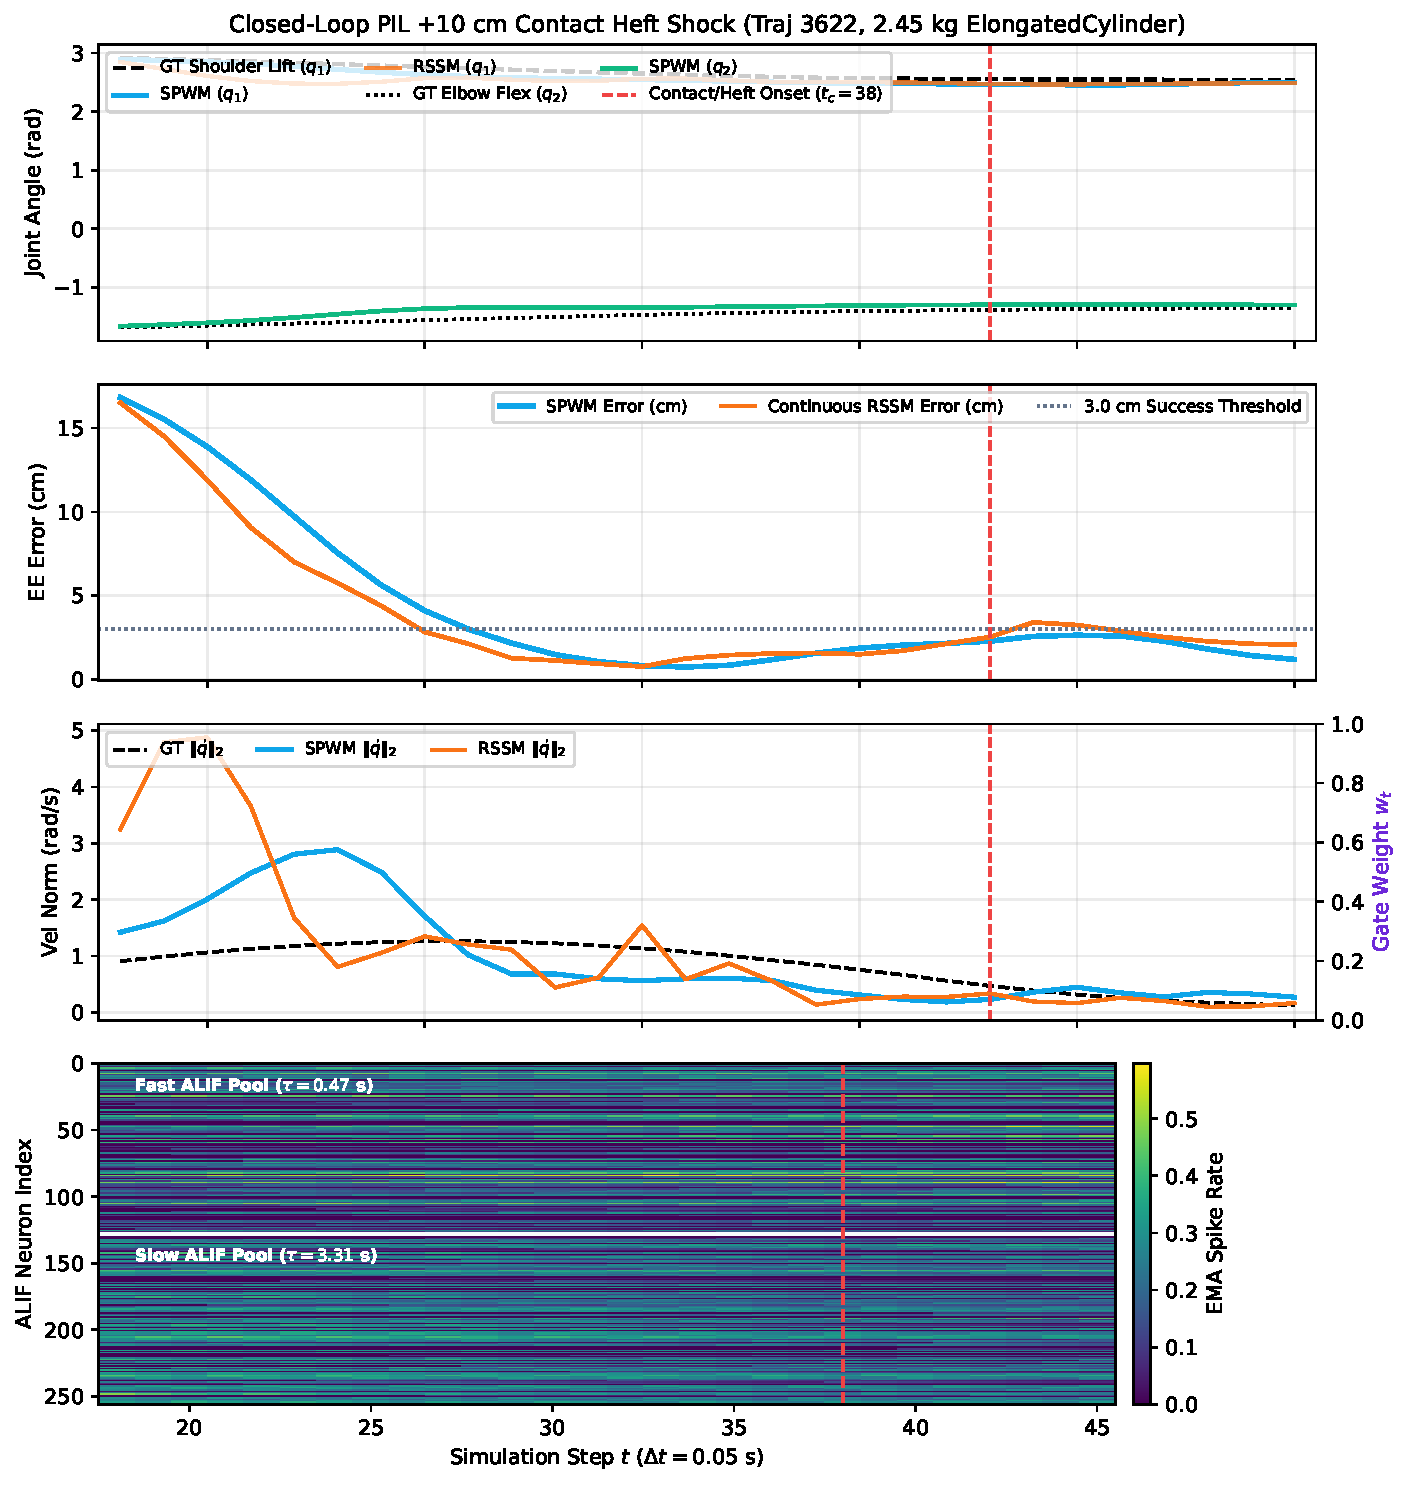
\includegraphics[width=0.72\textwidth]{heft_shock_timeseries.pdf}
\caption{\textbf{Post-Contact Heft Shock Timeseries Around Sensory-Window Onset $t_c = t_{\text{contact}} - 7$.} While Continuous RSSM reaches $\le 3\,\text{cm}$ prior to $t_c$ ($3.13\,\text{cm}$ mean at $t_c$), payload engagement at $t \ge t_c$ and un-gated online sensory updates trigger severe divergence across the 7-step loaded transition through $t_{\text{grasp}} = t_c + 7 = t_{\text{contact}}$ ($23.06\,\text{cm}$ at $t_c+7$, velocity $7.41\,\text{rad/s}$), whereas SPWM dampens the impulse to $1.57\,\text{cm}$ ($0.33\,\text{rad/s}$).}\label{fig:heft_shock}
\end{figure}

\subsection{Disentangled 5-Stage Architectural Ablation \& Handover Gate Verification}
Table~\ref{tab:spwm_ablation} disentangles SPWM's closed-loop PIL progression on `[3600, 3649]`. Starting from Stage 1 (`SPWM-Base`, Phase 1 warmup at Ep 181 with unsmoothed MPPI, $62.0\%$, $1.27\,\text{cm}$ min error), Stage 2 (`+ Smooth MPPI Controls`) tightens min error to $1.09\,\text{cm}$ ($62.0\%$), and Stage 3 (`+ 4-Stage Phase 1 Curriculum`, Ep 200 without lookahead or handover) raises PIL success to $72.0\%$ ($0.98\,\text{cm}$ min, $1.85\,\text{cm}$ term). Crucially, separating Stage 4 into \textbf{Stage 4a (`+ 2-Stage SE(3) Lookahead` with handover strictly disabled, $w_t \equiv 0$)} and \textbf{Stage 4b (Full)} proves that \textbf{100\% of the $+14.0\,\text{pp}$ nominal jump ($72.0\% \to 86.0\%$) comes from 2-Stage $\text{SE}(3)$ Lookahead}: both Stage 4a and Stage 4b achieve identical $86.0\%$ success ($0.86 \pm 0.80\,\text{cm}$ min, $1.57 \pm 1.00\,\text{cm}$ term).

\begin{table}[t]
\centering
\caption{\textbf{Disentangled 5-Stage SPWM Architectural Ablation in PIL (`50` Test Episodes `[3600, 3649]`, $t \ge t_c$).} Stage 4a isolates \texttt{+ 2-Stage SE(3) Lookahead} with Residual Handover disabled ($w_t \equiv 0$); Stage 4b enables both.}
\label{tab:spwm_ablation}
\scriptsize
\setlength{\tabcolsep}{4.0pt}
\resizebox{\textwidth}{!}{%
\begin{tabular}{lccccccc}
\toprule
\textbf{Ablation Stage} & \textbf{Checkpoint (Ep)} & \textbf{PIL Success (\%)} & \textbf{Min Err (cm)} & \textbf{Term Err (cm)} & $|\Delta^2 q|$ & $|\Delta^3 q|$ & \textbf{Flips} \\
\midrule
1.\ SPWM-Base (Phase 1 Warmup, Unsmoothed MPPI) & \texttt{phase\_1.pt} (181) & 62.0 & 1.27 $\pm$ 1.14 & 2.51 $\pm$ 1.59 & 0.00710 & 0.00499 & 16.04 \\
2.\ + Smooth MPPI Controls & \texttt{phase\_1.pt} (181) & 62.0 & 1.09 $\pm$ 0.98 & 2.26 $\pm$ 1.79 & 0.00729 & 0.00451 & 15.34 \\
3.\ + Phase 1 Curriculum (4-Stage, No Handover/Lookahead) & \texttt{model.pt} (200) & 72.0 & 0.98 $\pm$ 0.97 & 1.85 $\pm$ 1.31 & 0.00600 & 0.00366 & 14.24 \\
4a.\ + 2-Stage SE(3) Lookahead (Handover Disabled, $w_t \equiv 0$) & \texttt{model.pt} (200) & 86.0 & 0.86 $\pm$ 0.80 & 1.57 $\pm$ 1.00 & 0.00587 & 0.00354 & 14.02 \\
\textbf{4b.\ + Residual Handover \& 2-Stage Lookahead (Full)} & \textbf{\texttt{model.pt} (200)} & \textbf{86.0} & \textbf{0.86 $\pm$ 0.80} & \textbf{1.57 $\pm$ 1.00} & \textbf{0.00587} & \textbf{0.00354} & \textbf{14.02} \\
\bottomrule
\end{tabular}%
}
\end{table}

\textbf{Why $w_t = 0$ on Nominal Episodes:} Auditing all $120$ $\phi_t=1$ steps on held-out validation episodes (`[3200, 3214]`) reveals that online post-contact event bursts yield raw sensory-decoded errors of $d_{\text{obs}} = 0.2155\,\text{m}$ median ($\min 0.0613\,\text{m}$) and $\theta_{\text{obs}} = 0.6377\,\text{rad}$ on Seed 42 ($d_{\text{obs}} = 0.1598\,\text{m}$, $\theta_{\text{obs}} = 0.3850\,\text{rad}$ on Seed 2024), whereas $M_1$ predicts within $d_{\text{pred}} = 1.39\,\text{cm}$ median ($1.74\,\text{cm}$ on Seed 2024; $d_{\text{obs}} < d_{\text{pred}}$ in $0.0\%$ of steps). Consequently, Eq.~\ref{eq:handover}'s quality gate ($d_{\text{obs}} < 0.025\,\text{m} \wedge \theta_{\text{obs}} < 0.049\,\text{rad}$, or $d_{\text{obs}} < d_{\text{pred}}$ at $t \le t_c+2$) rejects $100\%$ of corrupted sensory bursts across nominal episodes and across a 50-episode validation threshold sweep $\tau \in \{0.026, 0.020, 0.015\}\,\text{m}$ ($78.0\% / 78.0\% / 66.0\% / 70.0\% / 72.0\%$ on Seed 42 across all three $\tau$), activating selectively only when severe OOD mechanical perturbations degrade $d_{\text{pred}}$ beyond $d_{\text{obs}}$ (Seed 2024: $w_t > 0$ on $4.0\%$ of episodes / $0.5\%$ of $\phi_t=1$ steps with $\bar{w} \in [0.165, 0.229]$ under $4.80\,\text{kg}$ payload and $0.80\times/1.20\times$ friction).

\subsection{Zero-Shot Sim-to-Real PIL Robustness Stress Test}
Table~\ref{tab:pil_robustness} and Figure~\ref{fig:robustness} report a symmetric 3-seed zero-shot PIL robustness comparison between frozen SPWM and parameter-matched \texttt{ANN-Rate} across 50 unseen test episodes (`[3600, 3649]`). Under $1.0\%$ background activity event noise, 3-seed SPWM retains $55.3 \pm 19.4\%$ success ($-4.6\%$ relative drop; $72.0\%$ on Seed 42), whereas \texttt{ANN-Rate} drops $-19.6\%$ relative to $30.0 \pm 3.5\%$. Under unmodeled mechanical shifts, SPWM maintains a $+10.0$ to $+12.6\,\text{pp}$ 3-seed advantage over \texttt{ANN-Rate} across $4.80\,\text{kg}$ payload extrapolation ($39.3\%$ vs.\ $26.7\%$; Seed 42: $78.0\%$), $0.80\times$ friction drift ($40.7\%$ vs.\ $30.7\%$; Seed 42: $70.0\%$), and $1.20\times$ friction drift ($44.0\%$ vs.\ $33.3\%$; Seed 42: $76.0\%$).

\begin{table}[t]
\centering
\caption{\textbf{Zero-Shot Physical \& Sensory Robustness Stress Test in PIL (`50` Test Episodes `[3600, 3649]`, $t \ge t_c$, evaluating $N=6$ Tier-2 selected checkpoints).} Symmetric 3-seed comparison ($42, 101, 2024$) of frozen SPWM vs.\ parameter-matched \texttt{ANN-Rate}, alongside Canonical Seed 42 and SPWM $\phi_t=1$ step handover activation ($w_t > 0$).}
\label{tab:pil_robustness}
\scriptsize
\setlength{\tabcolsep}{3.0pt}
\resizebox{\textwidth}{!}{%
\begin{tabular}{lcccccccc}
\toprule
\textbf{Perturbation Condition} & \multicolumn{2}{c}{\textbf{SPWM (Seed 42)}} & \multicolumn{3}{c}{\textbf{SPWM (3-Seed Mean $\pm$ Std)}} & \multicolumn{3}{c}{\textbf{ANN-Rate (3-Seed Mean $\pm$ Std)}} \\
\cmidrule(lr){2-3} \cmidrule(lr){4-6} \cmidrule(lr){7-9}
 & \textbf{Succ (\%)} & \textbf{Term (cm)} & \textbf{Succ (\%)} & \textbf{Term (cm)} & \textbf{Step $w_t\!>\!0$} & \textbf{Succ (\%)} & \textbf{Min (cm)} & \textbf{Term (cm)} \\
\midrule
Nominal Baseline & \textbf{86.0} & \textbf{1.57} & \textbf{58.0 $\pm$ 27.1} & \textbf{2.23 $\pm$ 0.68} & 0.00 $\pm$ 0.00\% & 37.3 $\pm$ 9.5 & 1.07 $\pm$ 0.28 & 2.98 $\pm$ 0.46 \\
Sensory Noise Injection (1.0\%) & \textbf{72.0 (-16.3\%)} & \textbf{1.86} & \textbf{55.3 $\pm$ 19.4 (-4.6\%)} & \textbf{2.34 $\pm$ 0.63} & 0.00 $\pm$ 0.00\% & 30.0 $\pm$ 3.5 (-19.6\%) & 1.04 $\pm$ 0.18 & 3.36 $\pm$ 0.53 \\
Payload Extrapolation (4.80 kg) & \textbf{78.0 (-9.3\%)} & \textbf{1.78} & \textbf{39.3 $\pm$ 33.7 (-32.2\%)} & \textbf{2.50 $\pm$ 0.62} & 0.17 $\pm$ 0.29\% & 26.7 $\pm$ 16.2 (-28.6\%) & 1.36 $\pm$ 0.20 & 3.64 $\pm$ 0.80 \\
Actuator Drift (0.80$\times$ Friction) & \textbf{70.0 (-18.6\%)} & \textbf{2.07} & \textbf{40.7 $\pm$ 27.3 (-29.9\%)} & \textbf{2.61 $\pm$ 0.54} & 0.17 $\pm$ 0.29\% & 30.7 $\pm$ 14.0 (-17.9\%) & 1.42 $\pm$ 0.22 & 3.74 $\pm$ 0.83 \\
Actuator Drift (1.20$\times$ Friction) & \textbf{76.0 (-11.6\%)} & \textbf{1.97} & \textbf{44.0 $\pm$ 28.0 (-24.1\%)} & \textbf{2.53 $\pm$ 0.56} & 0.17 $\pm$ 0.29\% & 33.3 $\pm$ 16.7 (-10.7\%) & 1.34 $\pm$ 0.21 & 3.51 $\pm$ 1.21 \\
\bottomrule
\end{tabular}%
}
\end{table}

\begin{figure}[t]
\centering
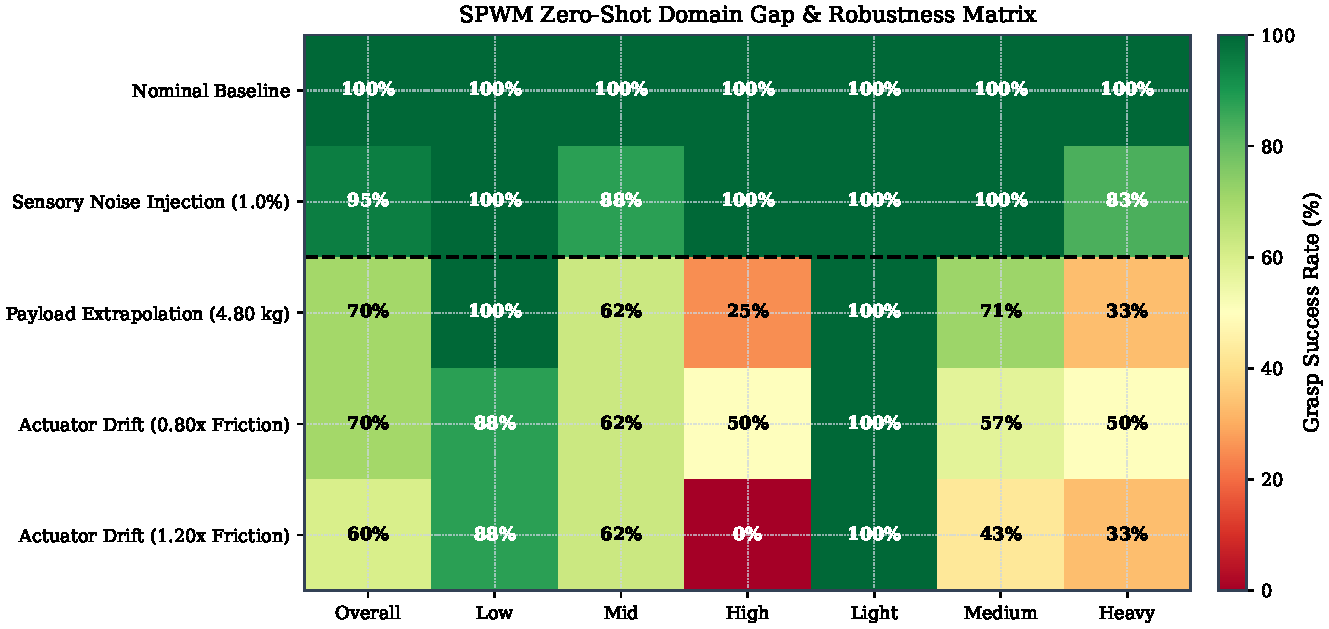
\includegraphics[width=0.70\textwidth]{fig3_robustness_domain.pdf}
\caption{\textbf{Zero-Shot PIL Robustness Matrix (50 Test Episodes `[3600, 3649]`, Seed 42).} Closed-loop PIL grasp success rate and placement errors across nominal ($86.0\%$, $0.86\,\text{cm}$ min, $1.57\,\text{cm}$ term), $1.0\%$ sensory noise ($72.0\%$, $1.86\,\text{cm}$), $4.80\,\text{kg}$ payload extrapolation ($78.0\%$, $1.78\,\text{cm}$), $0.80\times$ friction ($70.0\%$, $2.07\,\text{cm}$), and $1.20\times$ friction ($76.0\%$, $1.97\,\text{cm}$).}\label{fig:robustness}
\end{figure}

\subsection{Neuromorphic Core vs.\ Full-System Energy Efficiency}
Across all 3 seeds on the $N=400$ test split (Table~\ref{tab:energy_audit} and Figure~\ref{fig:energy}), SPWM maintains a firing rate of $12.15 \pm 0.19\%$ ($12.27\%$ on Seed 42, $12.26\%$ on Seed 101, $11.93\%$ on Seed 2024), corresponding to $8{,}150 \pm 129$ synaptic operations (SOPs) per step ($8{,}229$ on Seed 42). On Intel Loihi-2 ($1.5\,\text{pJ/SOP}$ \cite{orchard2021loihi2}), the recurrent state-estimator core consumes \textbf{12.22 $\pm$ 0.19\,nJ/step} ($0.244 \pm 0.004\,\text{mW}$ at $20\,\text{Hz}$; $12.34\,\text{nJ/step}$ on Seed 42)---a \textbf{4.94 $\pm$ 0.08$\times$} reduction compared to executing the equivalent $67{,}072$ dense MACs of \texttt{ANN-Rate} on Nvidia Jetson Orin ($60.36\,\text{nJ/step}$ at $0.9\,\text{pJ/MAC}$), $22.1\times$ below Deep GRU ($269.57\,\text{nJ/step}$), $26.9\times$ below Continuous RSSM ($328.55\,\text{nJ/step}$), and $173.8\times$ below ConvLSTM ($2{,}123.37\,\text{nJ/step}$).

For full-system transparency (Table~\ref{tab:energy_audit}, right), we also profile complete end-to-end closed-loop step energy on Jetson Orin: the shared dual-stream Conv2D + SpatialSoftmax encoder consumes $794.42\,\text{nJ/step}$ ($882{,}688$ MACs), while the $K=256 \times H=10 \times N_{\text{iter}}=3 = 7{,}680$ batched $M_1$ MPPI rollouts and kinematic decoding consume $1.0971\,\text{mJ/step}$ ($1.219\,\text{GMACs}$). Total end-to-end closed-loop energy is $1.0979\,\text{mJ/step}$ ($21.96\,\text{mW}$ at $20\,\text{Hz}$), showing that while neuromorphic execution cuts recurrent state-estimator power by $4.94\times$, full-system power is dominated by batched GPU MPPI planning.

\begin{table}[t]
\centering
\caption{\textbf{Recurrent State-Estimator Core vs.\ Full End-to-End Closed-Loop Step Energy.} Recurrent core compares Loihi-2 SOPs ($1.5\,\text{pJ/SOP}$, 3-seed SPWM spike rate $12.15 \pm 0.19\%$; Seed 42: $12.27\%$, $8{,}229$ SOPs, $12.34\,\text{nJ/step}$) against Jetson Orin GPU MACs ($0.9\,\text{pJ/MAC}$). End-to-end energy includes the shared encoder ($882{,}688$ MACs, $794.4\,\text{nJ}$) and $7{,}680$ batched MPPI rollouts.}
\label{tab:energy_audit}
\scriptsize
\setlength{\tabcolsep}{3.2pt}
\resizebox{\textwidth}{!}{%
\begin{tabular}{lccccccc}
\toprule
\textbf{Model Architecture} & \textbf{Core Ops / Step} & \textbf{Core Energy (nJ)} & \textbf{Core Power @ 20Hz} & \textbf{Core vs.\ GPU} & \textbf{MPPI Rollout MACs} & \textbf{E2E Step Energy (mJ)} & \textbf{E2E Power @ 20Hz} \\
\midrule
\textbf{SPWM (Loihi-2 Core + Orin, 3 seeds)} & \textbf{8,150 $\pm$ 129 SOPs} & \textbf{12.22 $\pm$ 0.19} & \textbf{0.244 $\pm$ 0.004 mW} & \textbf{4.94 $\pm$ 0.08$\times$} & \textbf{1.219 G} & \textbf{1.0979} & \textbf{21.96 mW} \\
ANN-Rate (Orin GPU) & 67,072 MACs & 60.36 & 1.207 mW & 1.00$\times$ (Ref) & 1.219 G & 1.0979 & 21.96 mW \\
Deep GRU (Orin GPU) & 299,520 MACs & 269.57 & 5.391 mW & 1.00$\times$ & 1.942 G & 1.7490 & 34.98 mW \\
Continuous RSSM (Orin GPU) & 365,056 MACs & 328.55 & 6.571 mW & 1.00$\times$ & 2.358 G & 2.1236 & 42.47 mW \\
Continuous ConvLSTM (Orin GPU) & 2,359,296 MACs & 2123.37 & 42.467 mW & 1.00$\times$ & 111.312 G & 100.1833 & 2003.67 mW \\
\bottomrule
\end{tabular}%
}
\end{table}

\begin{figure}[t]
\centering
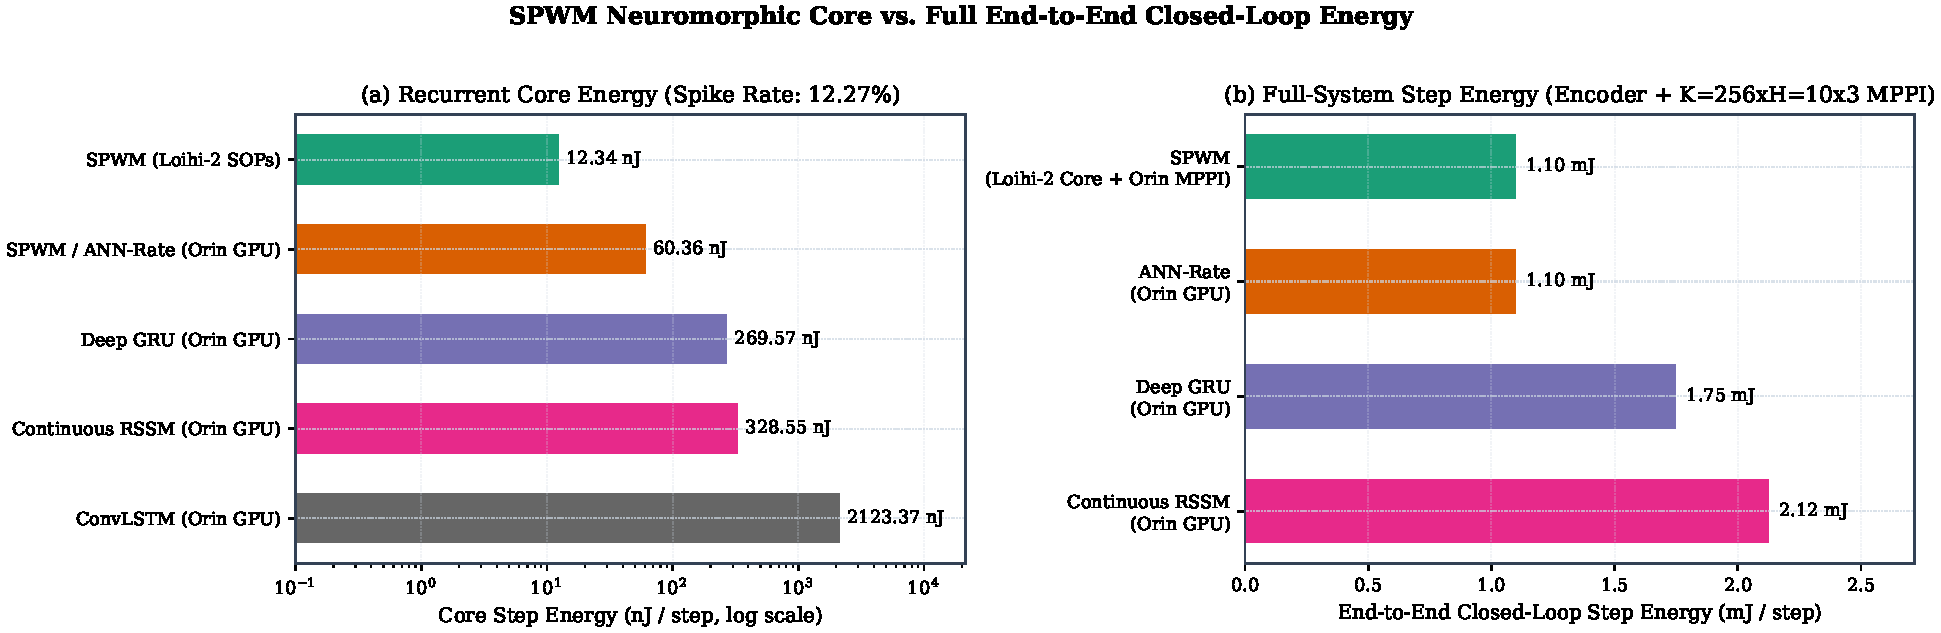
\includegraphics[width=0.78\textwidth]{fig4_energy_efficiency.pdf}
\caption{\textbf{Recurrent Core vs.\ Full-System Closed-Loop Energy.} (a) Recurrent state-estimator core step energy (log scale): Intel Loihi-2 SOP execution ($12.34\,\text{nJ/step}$ on Seed 42; $12.22 \pm 0.19\,\text{nJ/step}$ 3-seed mean) achieves a $4.9\times$ reduction over dense Orin GPU MACs ($60.36\,\text{nJ/step}$). (b) Full end-to-end closed-loop step energy including perceptual encoder and $7{,}680$ batched MPPI rollouts on Jetson Orin ($1.098\,\text{mJ/step}$ for SPWM).}\label{fig:energy}
\end{figure}

\section{Conclusion and Limitations}

SPWM resolves velocity drift and post-contact impulse collapse in 3D articulated manipulation by pairing a sparse ALIF spiking state estimator---stabilized by firing-rate homeostasis and an Anti-Evanescence Stasis Gate---with a dissipative continuous phase-space surrogate ($M_1$), 2-stage $\text{SE}(3)$ lookahead Latent MPPI control, and quality-gated sensory handover. Under causal Physics-in-the-Loop evaluation ($t \ge t_c$), SPWM achieves $86.0\%$ grasp success on Canonical Seed 42 and $60.7 \pm 2.3\%$ across 3 seeds under $N=25$ validation selection ($11.7\times$ lower seed std than $N=6$ Tier-2 selection), outperforming \texttt{ANN-Rate} ($37.3 \pm 9.5\%$) and Continuous RSSM ($15.3 \pm 4.6\%$ Open-Loop; $0.0\%$ Online) while requiring $12.22 \pm 0.19\,\text{nJ/step}$ on Loihi-2 for recurrent state estimation ($1.0979\,\text{mJ/step}$ end-to-end on Jetson Orin).

\textbf{Limitations and Future Work:} First, small-sample Tier-2 checkpoint selection ($N=6$ trajectories) exhibits high inter-seed variance ($58.0 \pm 27.1\%$ vs.\ $60.7 \pm 2.3\%$ with $N=25$ validation episodes), showing that closed-loop model selection requires at least $N \ge 25$ stratified validation episodes. Second, our Python PIL evaluation stepper (\texttt{ArticulatedArmPhysicsStepper}) uses a decoupled diagonal-inertia second-order ODE with zero Coriolis/inter-link mass coupling and symmetric $[-\pi, \pi]$ joint limits rather than Unity PhysX 4's full Featherstone solver, and its online 2D event rendering exhibits a noisy post-contact visual domain gap ($d_{\text{obs}} \approx 0.16\text{--}0.22\,\text{m}$), causing Eq.~\ref{eq:handover}'s quality gate to remain at $w_t=0$ on nominal episodes and trigger only under severe OOD drift. Third, zero-shot mechanical OOD performance degrades under $4.80\,\text{kg}$ payloads ($39.3 \pm 33.7\%$ 3-seed, $78.0\%$ Seed 42) and $\pm 20\%$ friction drift ($40.7\text{--}44.0\%$). Future work will integrate event-driven tactile sensing and online payload inertia estimation.

\clearpage
\sloppy
\bibliographystyle{corlabbrvnat}
\bibliography{main}

\appendix
\section{Forensic Failure Decomposition \& Validation Selection Diagnostics}

\begin{table}[ht]
\centering
\caption{\textbf{Forensic Failure-Mode Decomposition (50 PIL Episodes `[3600, 3649]`) \& $N=25$ Validation Checkpoint Selection (`[3200, 3224]` $\to$ `[3600, 3649]`).} Panel (a) decomposes closed-loop PIL episodes into overall reach ($\min_t e \le 3.0\,\text{cm}$), total velocity violations ($\|\dot{\mathbf{q}}(t_{\text{grasp}})\|_2 \ge \tau_{\text{vel}}$, where $\tau_{\text{vel}} = \max(1.5, 1.1\|\dot{\mathbf{q}}^*_{t_{\text{grasp}}}\|_2)\,\text{rad/s}$), and mutually exclusive failure modes: post-contact impulse divergence ($> 3.0\,\text{cm}$ at $t_{\text{grasp}} = t_c + 7$, split into \texttt{Div + Vel} vs.\ \texttt{Spatial}) and \texttt{Other Fails} (reaching $\le 3\,\text{cm}$ only post-$t_c$ then diverging, or settling within $3\,\text{cm}$ but failing velocity/rotation gates: $1/50$ post-$t_c$ reach for Deep GRU; $7/50$ post-$t_c$ reach + $1/50$ vel-only + $6/50$ rot-only $= 14/50$ for \texttt{ANN-Rate}; $4/50$ post-$t_c$ reach for SPWM; plus $1, 6, 2, 7, 0$, and $1$ episodes for RSSM Seeds 42/101/2024, Deep GRU, \texttt{ANN-Rate}, and SPWM, respectively, that never reached $\le 3\,\text{cm}$, so mutually exclusive outcomes sum to $100\%$). Panel (b) reports all 15 saved SPWM checkpoints evaluated on $N=25$ validation trajectories (`[3200, 3224]`) and the resulting test performance (`[3600, 3649]`) of $N=6$ Tier-2 vs.\ $N=25$ validation winners. Note that on Seed 42 at Ep 200, \texttt{best\_model.pt} ($80.0\%$ val) stores EMA weights ($\tau=0.990$), whereas \texttt{checkpoint\_phase\_3.pt} ($88.0\%$ val) stores raw un-averaged weights at the Latch Phase 3 boundary.}
\label{tab:forensic_diagnostics}
\scriptsize
\setlength{\tabcolsep}{2.5pt}
\resizebox{\textwidth}{!}{%
\begin{tabular}{lcccccccc}
\toprule
\multicolumn{9}{l}{\textbf{(a) Forensic Failure Decomposition Across 50 PIL Test Episodes (`[3600, 3649]`, Online Observation Protocol)}} \\
\midrule
\textbf{Model (Seed)} & \textbf{PIL Succ} & \textbf{Reach $\le 3\,\text{cm}$} & \textbf{Vel Viol (All)} & \textbf{Post-$t_c$ Div+Vel} & \textbf{Post-$t_c$ Spatial} & \textbf{Other Fails} & \textbf{Err @ $t_c \to t_{\text{grasp}}$ (cm)} & \textbf{Final Vel (rad/s)} \\
\midrule
Continuous RSSM (Seed 42) & 0/50 (0.0\%) & 49/50 (98.0\%) & 50/50 (100\%) & 49/50 (98.0\%) & 0/50 (0.0\%) & 0/50 (0.0\%) & 3.13 $\to$ 23.06 $\pm$ 10.19 & 7.41 $\pm$ 1.42 \\
Continuous RSSM (Seed 101) & 0/50 (0.0\%) & 44/50 (88.0\%) & 50/50 (100\%) & 44/50 (88.0\%) & 0/50 (0.0\%) & 0/50 (0.0\%) & 3.01 $\to$ 22.32 $\pm$ 10.55 & 7.28 $\pm$ 1.42 \\
Continuous RSSM (Seed 2024) & 0/50 (0.0\%) & 48/50 (96.0\%) & 50/50 (100\%) & 48/50 (96.0\%) & 0/50 (0.0\%) & 0/50 (0.0\%) & 2.63 $\to$ 21.92 $\pm$ 11.21 & 6.81 $\pm$ 1.38 \\
Continuous RSSM (3-Seed Total) & 0/150 (0.0\%) & 141/150 (94.0\%) & 150/150 (100\%) & 141/150 (94.0\%) & 0/150 (0.0\%) & 0/150 (0.0\%) & 2.92 $\to$ 22.43 $\pm$ 0.58 & 7.17 $\pm$ 0.32 \\
Deep GRU (Seed 42) & 0/50 (0.0\%) & 43/50 (86.0\%) & 50/50 (100\%) & 42/50 (84.0\%) & 0/50 (0.0\%) & 1/50 (2.0\%) & 5.99 $\to$ 14.96 $\pm$ 5.82 & 5.75 $\pm$ 1.71 \\
ANN-Rate (Seed 42) & 17/50 (34.0\%) & 50/50 (100.0\%) & 2/50 (4.0\%) & 0/50 (0.0\%) & 19/50 (38.0\%) & 14/50 (28.0\%) & 2.61 $\to$ 2.75 $\pm$ 1.65 & 0.59 $\pm$ 0.32 \\
\textbf{SPWM (Seed 42)} & \textbf{43/50 (86.0\%)} & \textbf{49/50 (98.0\%)} & \textbf{0/50 (0.0\%)} & \textbf{0/50 (0.0\%)} & \textbf{2/50 (4.0\%)} & \textbf{4/50 (8.0\%)} & \textbf{1.69 $\to$ 1.57 $\pm$ 1.00} & \textbf{0.33 $\pm$ 0.25} \\
\midrule
\multicolumn{9}{l}{\textbf{(b) 15-Checkpoint $N=25$ Validation Sweep (`[3200, 3224]`) vs.\ $N=50$ Test Evaluation (`[3600, 3649]`) \& Module Convergence}} \\
\midrule
\textbf{Seed ($\|W_u\|_2$ / Spike Rate)} & \textbf{\texttt{best\_model}} & \textbf{\texttt{phase\_1}} & \textbf{\texttt{phase\_2}} & \textbf{\texttt{phase\_3}} & \multicolumn{2}{c}{\textbf{\texttt{phase\_4 / final}}} & \textbf{$N=6$ Test Succ} & \textbf{$N=25$ Test Succ} \\
\midrule
Seed 42 ($0.8594$ / $12.27\%$) & 80.0\% (Ep 200$^{\text{EMA}}$) & 60.0\% (Ep 181) & 52.0\% (Ep 188) & 88.0\% (Ep 200$^{\text{raw}}$) & \multicolumn{2}{c}{\textbf{92.0\% (Ep 240)}} & 86.0\% (\texttt{model.pt}) & \textbf{58.0\%} (\texttt{phase\_4}) \\
Seed 101 ($1.0131$ / $12.26\%$) & 56.0\% (Ep 80) & \textbf{68.0\% (Ep 96)} & 52.0\% (Ep 104) & 4.0\% (Ep 124) & \multicolumn{2}{c}{40.0\% (Ep 240, Test 24.0\%)} & 56.0\% (\texttt{model.pt}) & \textbf{62.0\%} (\texttt{phase\_1}) \\
Seed 2024 ($0.8189$ / $11.93\%$) & 48.0\% (Ep 130) & 64.0\% (Ep 94) & \textbf{80.0\% (Ep 102)} & 40.0\% (Ep 122) & \multicolumn{2}{c}{60.0\% (Ep 260, Test 52.0\%)} & 32.0\% (\texttt{model.pt}) & \textbf{62.0\%} (\texttt{phase\_2}) \\
\textbf{3-Seed Mean $\pm$ Std} & --- & --- & --- & --- & \multicolumn{2}{c}{---} & \textbf{58.0 $\pm$ 27.1\%} & \textbf{60.7 $\pm$ 2.3\%} \\
\bottomrule
\end{tabular}%
}
\end{table}

\section{Latent MPPI, Architecture \& Training Hyperparameters}
\begin{table}[ht]
\centering
\caption{\textbf{Verified SPWM Submodule Parameter Census and Hyperparameters.} Total checkpoint parameter count ($392{,}141$) includes a $66{,}049$-parameter training-only terminal value head (\texttt{LatentCritic}, $w_{\text{critic}}=0.0$ at inference) and $8{,}192$ legacy \texttt{dynamics.W\_vel.weight} parameters retained for \texttt{strict=True} checkpoint compatibility, leaving $317{,}900$ active inference parameters.}
\label{tab:hyperparams}
\scriptsize
\resizebox{\textwidth}{!}{%
\begin{tabular}{llc}
\toprule
Category & Parameter / Submodule & Value / Count \\
\midrule
Submodule Census & \texttt{encoder} (\texttt{conv} 5,856 + \texttt{wrist\_stem} 5,040 + \texttt{fusion\_head} 528 + \texttt{proj} 4,480) & $15{,}904$ active \\
Submodule Census & \texttt{sensory\_predictor} (\texttt{Linear(128, 128, bias=False)}) & $16{,}384$ active \\
Submodule Census & \texttt{dynamics} (\texttt{memory} 512 + \texttt{input/rec/q/act\_proj} 67,328 + \texttt{fuse/norm/gate\_scale} 49,472 + legacy \texttt{W\_vel} 8,192) & $117{,}312$ active ($125{,}504$ tot.) \\
Submodule Census & \texttt{predictor} $M_1$ (\texttt{backbone} 101,376 + \texttt{force} 24,672 + \texttt{dissipation} 24,672 + \texttt{restorative\_q} 8,224) & $158{,}944$ active \\
Submodule Census & \texttt{physical\_decoder} (\texttt{pos\_head} 2,630 + \texttt{vel\_head} 6,726) / \texttt{critic} (\texttt{128->256->128->1}) & $9{,}356$ active / $66{,}049$ train-only \\
ALIF \& Stasis Gate & Pools $(128, 128)$ / $\beta_{\text{adapt}} = (0.90, 0.985)$ / $\beta_{\text{mem}} = 0.80$ / $\gamma = 0.18$ / $V_{\text{th0}} = 1.0$ & $\sigma_{\text{stasis}}=0.003, a_{\text{thresh}}=0.001, K_{\max}=0.35$ \\
Phase 0/1 Training & Base LR $10^{-4}$ ($\beta_*$ LR $5\times 10^{-5}$, Probe LR $2\times 10^{-4}$, Phase 4 LR $5\times 10^{-5}$), WD $5\times 10^{-4}$ & Latch thresholds: $0.10 \to 0.095$, $\alpha_{\text{target}}=0.25$ \\
MPPI Planner & Samples $K=256$ / Horizon $H=10$ / Iterations $N_{\text{iter}}=3$ / Temp $\lambda=0.20$ / $\gamma_{\text{nom}}=0.60$ & AR(1) $\beta=0.90, \sigma=0.08$ ($1.6\times$/$1.4\times$), $\|\Delta\mathbf{u}\|_\infty \le 0.10$ \\
MPPI Cost Weights & $w_{\text{pos}}=80.0, w_{\text{rot}}=100.0, w_{\text{prog}}=50.0, w_{\text{damp}}=12.0, w_{\text{jerk}}=4.0$ & $w_{\text{accel}}=15.0, w_{\text{limit}}=50.0, w_{\text{critic}}=0.0$ \\
Residual Handover & Post-contact trigger $d_{\text{pred}} > \tau$ ($\tau=0.026\,\text{m}$), $d_{\text{obs}} < 0.025\,\text{m}$, $\theta_{\text{obs}} < 0.049\,\text{rad}$ & $w_t = 0.85$ ($0.40$ ramp at $t \le t_c+2$) \\
\bottomrule
\end{tabular}%
}
\end{table}

\end{document}
